\documentclass[12pt]{beamer}
%\documentclass[20pt,handout]{beamer}
\usetheme{Darmstadt}
\usepackage{graphicx}
\usepackage[ngerman]{babel}
\usepackage[T1]{fontenc}
\usepackage[utf8]{inputenc}
\usepackage{tikz}
\usepackage[shadow,colorinlistoftodos]{todonotes}
\setbeamertemplate{footline}[frame number]

\newcommand{\cc}[1]{\includegraphics[height=4mm]{img/#1.png}}
\usepackage{ifthen}
\newcommand{\license}[2][]{\\#2\ifthenelse{\equal{#1}{}}{}{\\\scriptsize\url{#1}}}
\usepackage{textcomp}

%%% keine grauen Items in Listen  \setbeamercovered{transparent}

\pgfdeclareimage[height=.6cm]{c3d2logo}{./img/c3d2.pdf}

\pgfdeclarelayer{foreground}
\pgfsetlayers{main,foreground}
\logo{\pgfputat{\pgfxy(-1,0)}{\pgfbox[center,base]{\pgfuseimage{c3d2logo}}}}


\title{Chaos macht Schule}
\author{\small Robert Wartenberg \& Benjamin Partzsch\\\large Chaos Computer Club Dresden}
\date{26.06.2018}

\begin{document}
\maketitle

\section{Einleitung}
\subsection{}

\begin{frame}
	\frametitle{Hacker}
	\begin{figure}
	  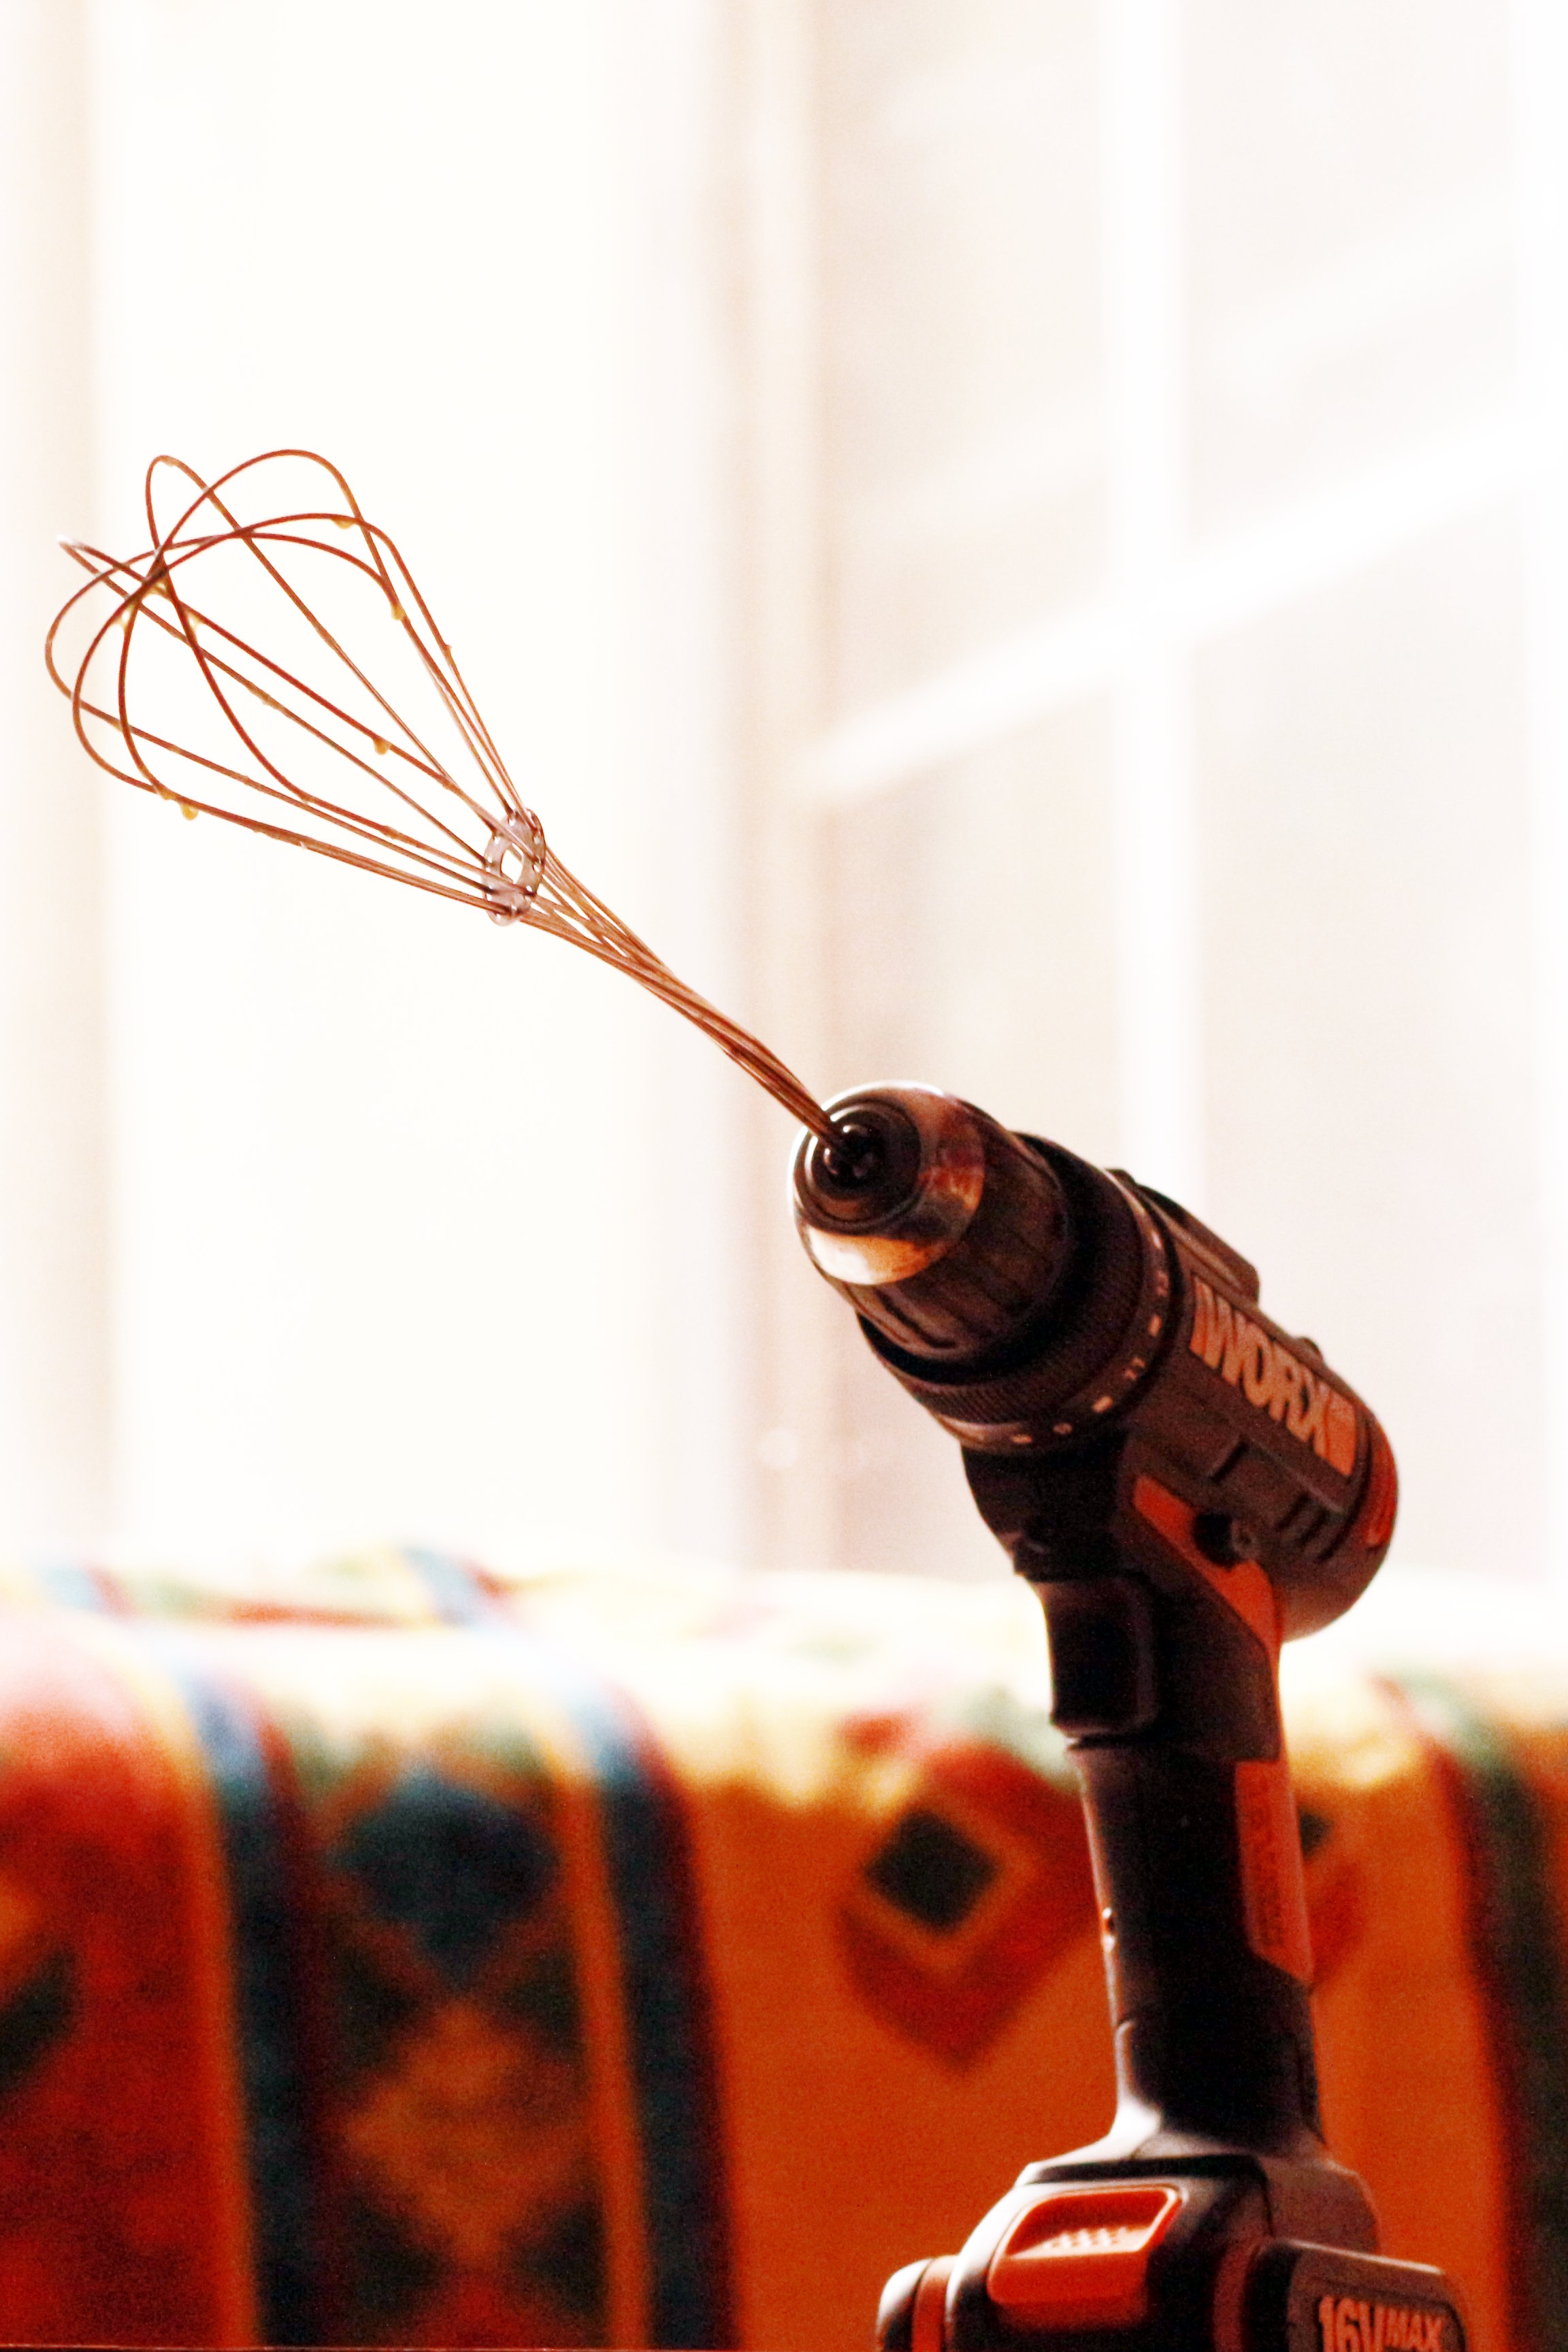
\includegraphics[height=0.7\textheight]{img/schneeschrauber.jpg}
	\end{figure}
  \end{frame}  


\begin{frame}
	\frametitle{Chaos Computer Club}
	\begin{center}
		
\includegraphics[height=0.2\textheight]{img/chaosknoten.png}
	\end{center}	
	\begin{itemize}
		\item<1-> Verein wurde 1981 gegründet (\url{https://ccc.de})          
		\item<2-> Aktuell mehr als 6000 Mitglieder
		\item<3-> Betreibt u.a. Öffentlichkeitsarbeit und Politikberatung      
		\item<4-> Lokale Erfahrungsaustauschkreise (Erfas) und Chaostreffs
	\end{itemize}
\end{frame}



\section{C3D2}
\subsection{}

\begin{frame}
	\frametitle{Chaos Computer Club Dresden}
	\begin{figure}
		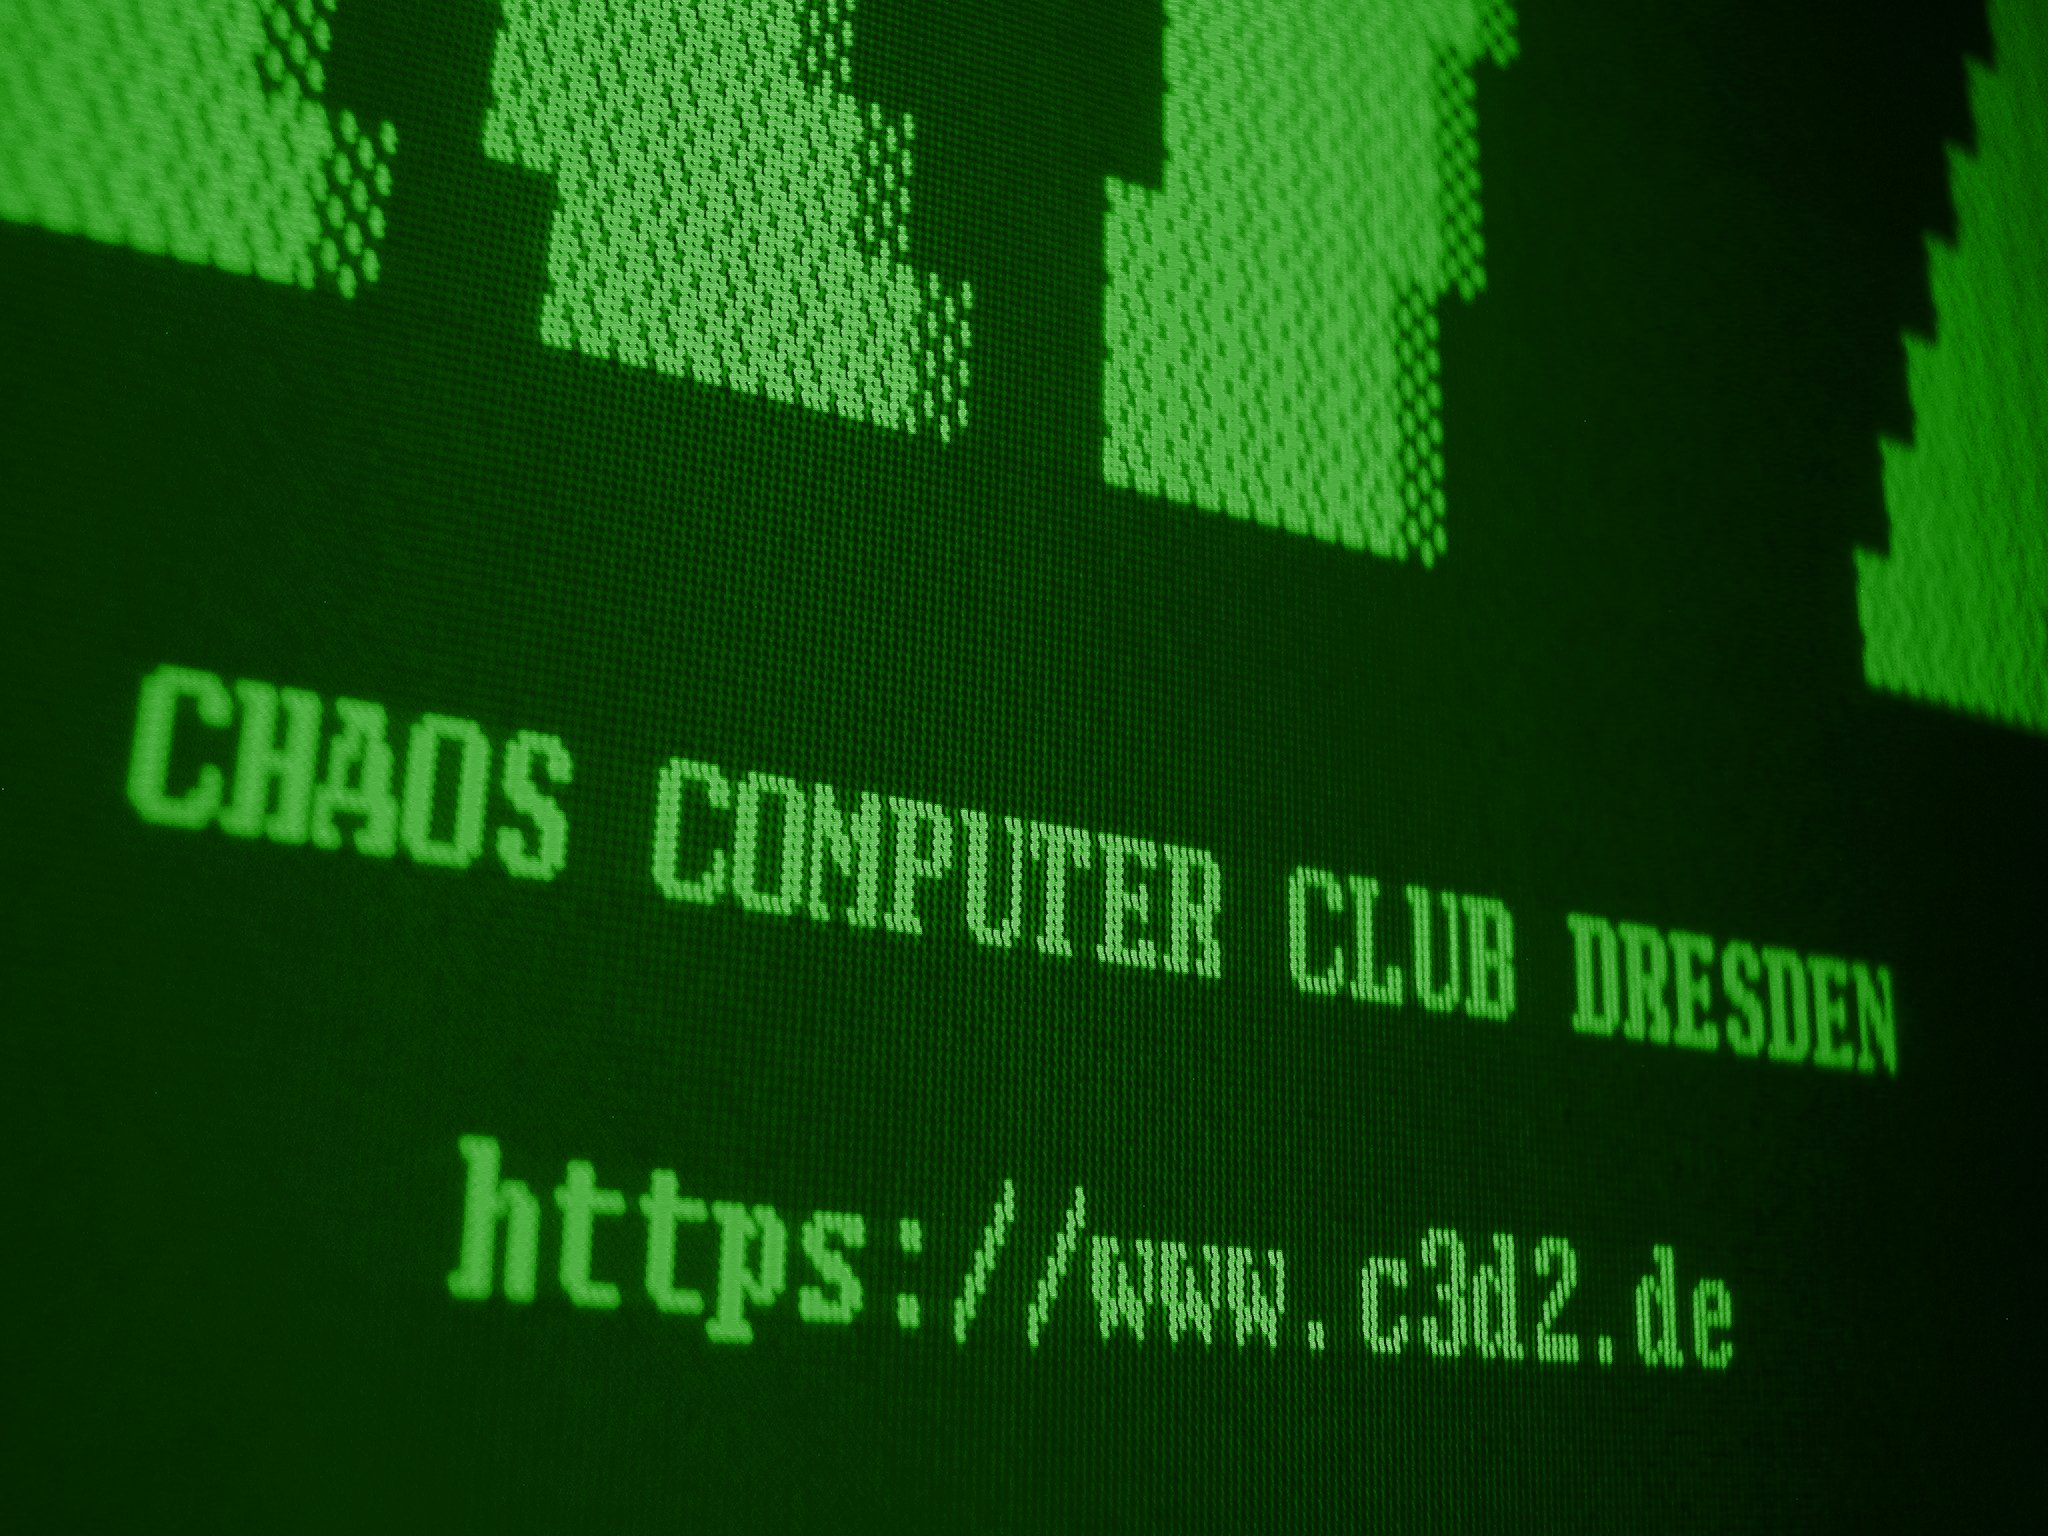
\includegraphics[height=0.7\textheight]{img/c3d2_green.jpg}
    \end{figure}
\end{frame}


\begin{frame}	
	\frametitle{Chaos Computer Club Dresden}
	\begin{center}
		Erfahrungsaustauschkreis Dresden
		\vspace{0.4cm}

		CCCDD
		\vspace{0.4cm}

		
\includegraphics[height=0.1\textheight]{img/c3d2_logo.png}		
		\vspace{0.4cm}

		https://c3d2.de

	\end{center}
\end{frame}	

\begin{frame}	
	\frametitle{Chaos Computer Club Dresden}
	\begin{center}
		Space to Hack, Make and drink Mate
		\vspace{0.4cm}

		\includegraphics[height=0.3\textheight]{img/c3d2-space-wide-180.jpg}
		
		\includegraphics[height=0.3\textheight]{img/c3d2-workshop-wide-180.jpg}
	\end{center}
\end{frame}	

\begin{frame}	
	\frametitle{Chaos Computer Club Dresden}
	\begin{center}
		Netzwerk
		\vspace{0.4cm}

		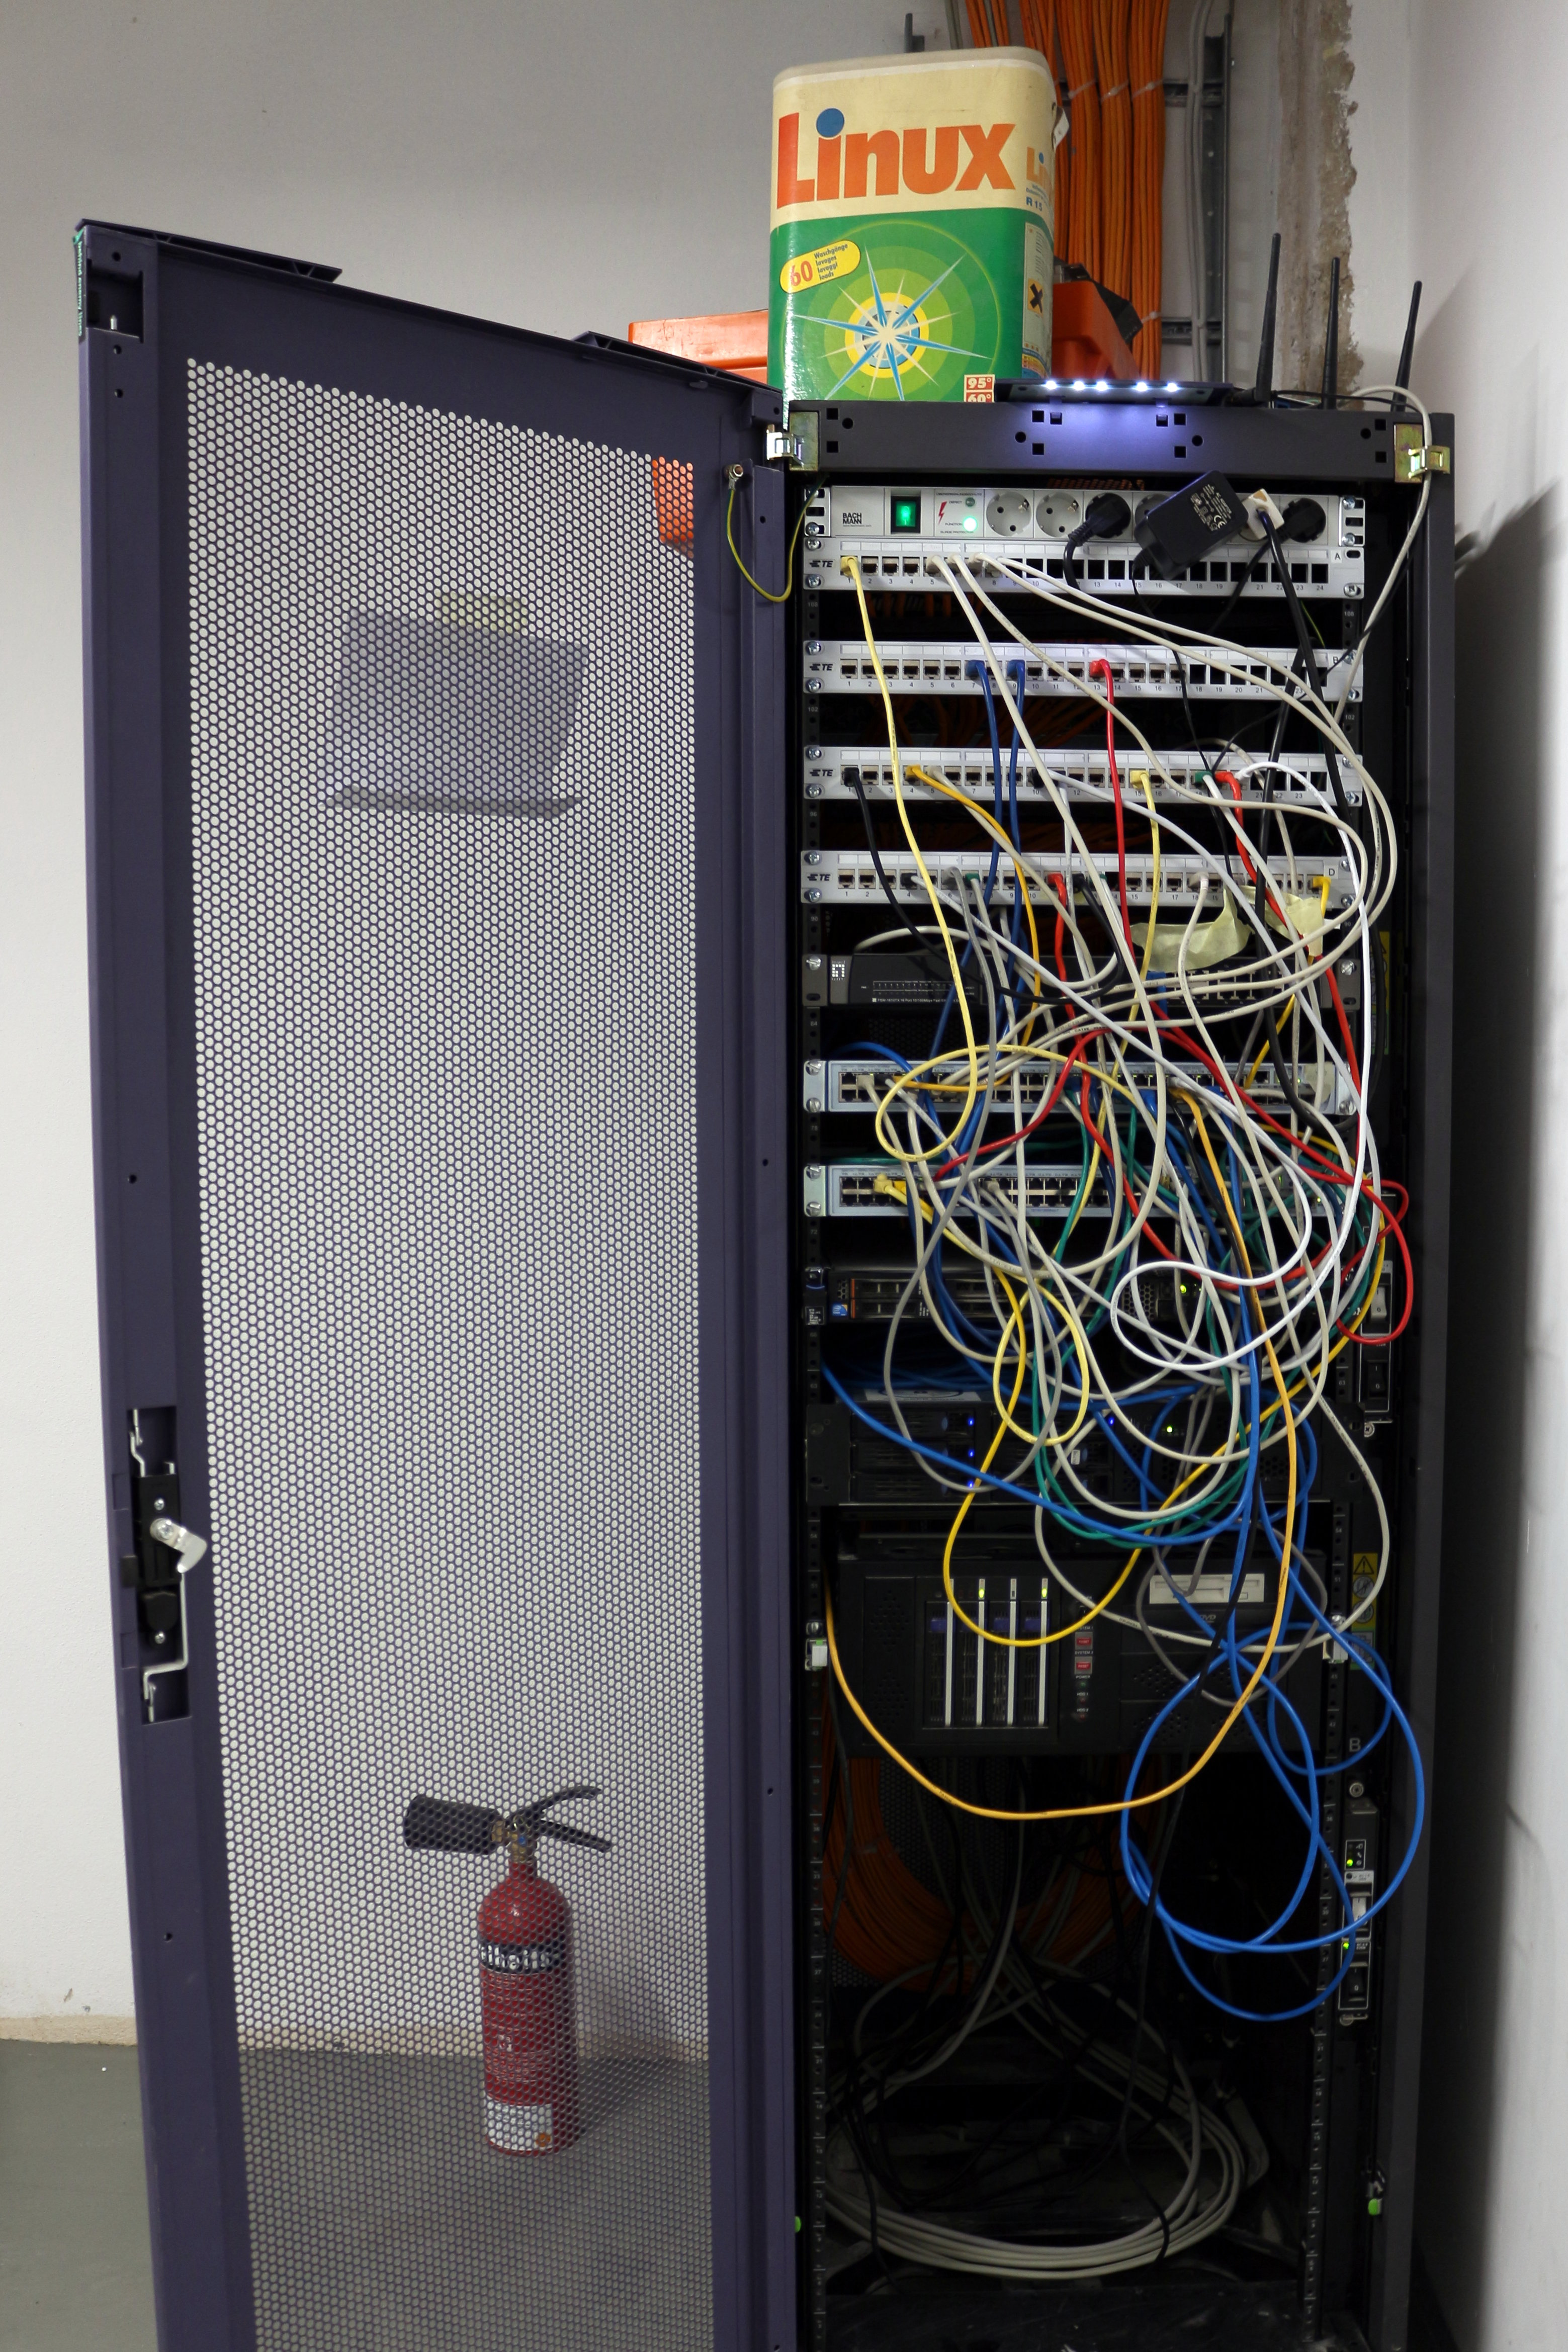
\includegraphics[height=0.6\textheight]{img/rack.jpg}
	\end{center}
\end{frame}	


\begin{frame}	
	\frametitle{Chaos Computer Club Dresden}
	\begin{center}
		Internet
		\vspace{0.4cm}	

		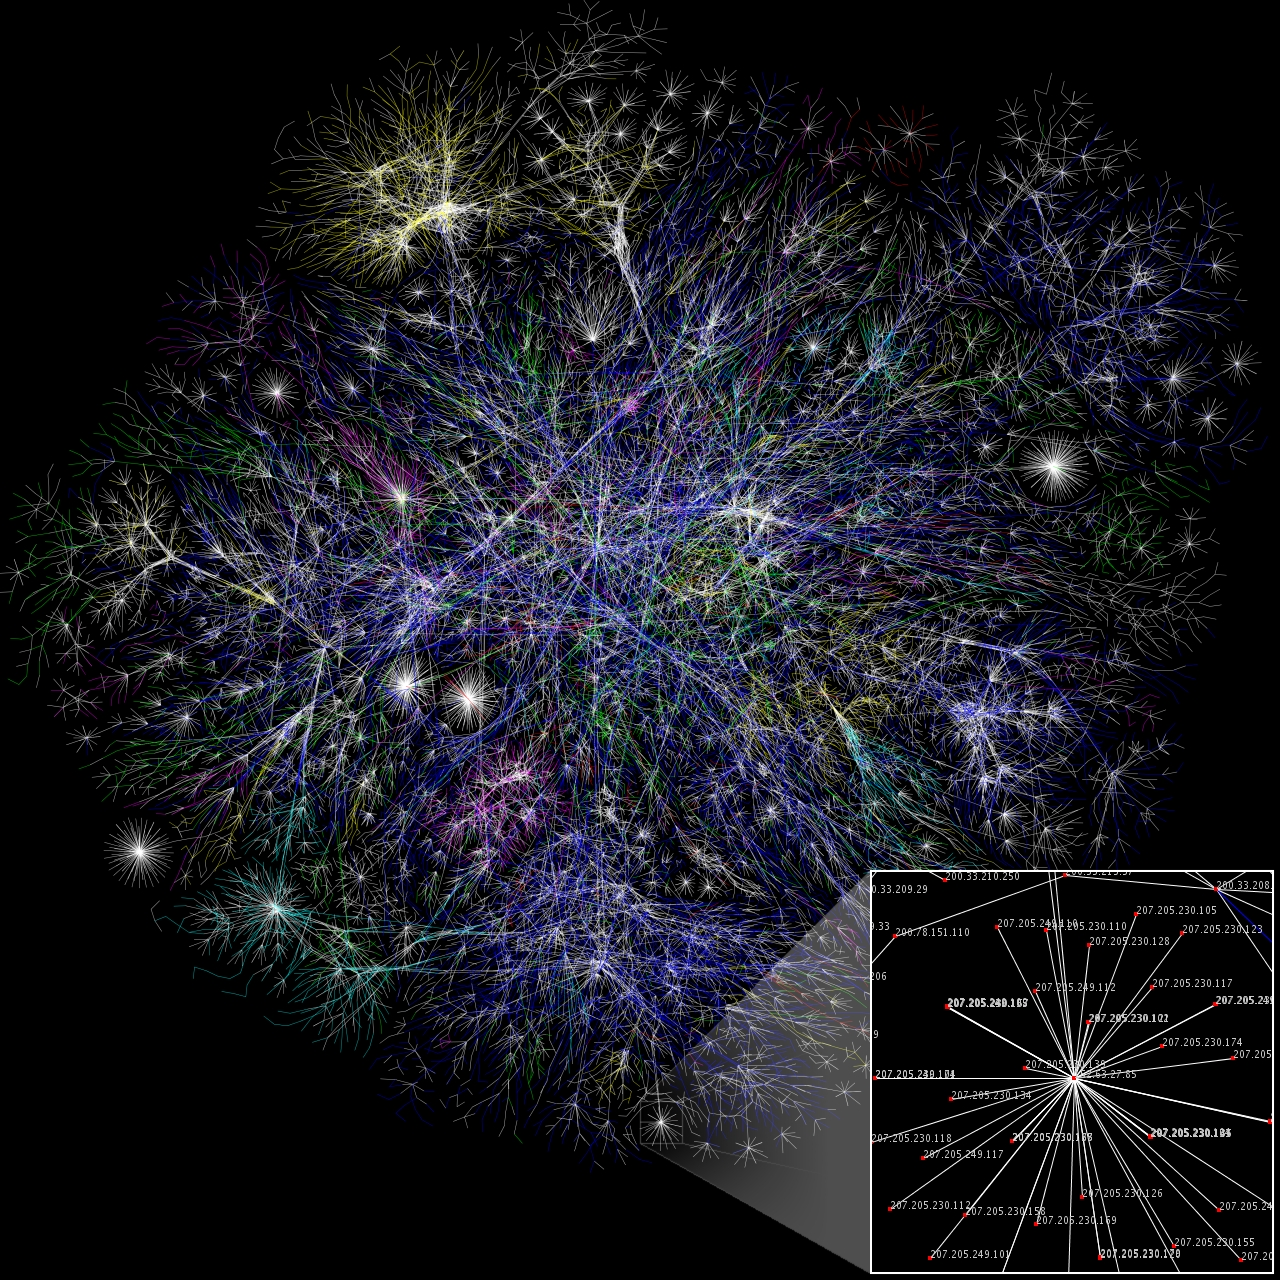
\includegraphics[height=0.6\textheight]{img/internet_0.jpg}
	\end{center}
\end{frame}	

\begin{frame}	
	\frametitle{Chaos Computer Club Dresden}
	\begin{center}
		
\includegraphics[height=0.2\textheight]{img/pentaradio.png}	
		\hspace{0.4cm}		
		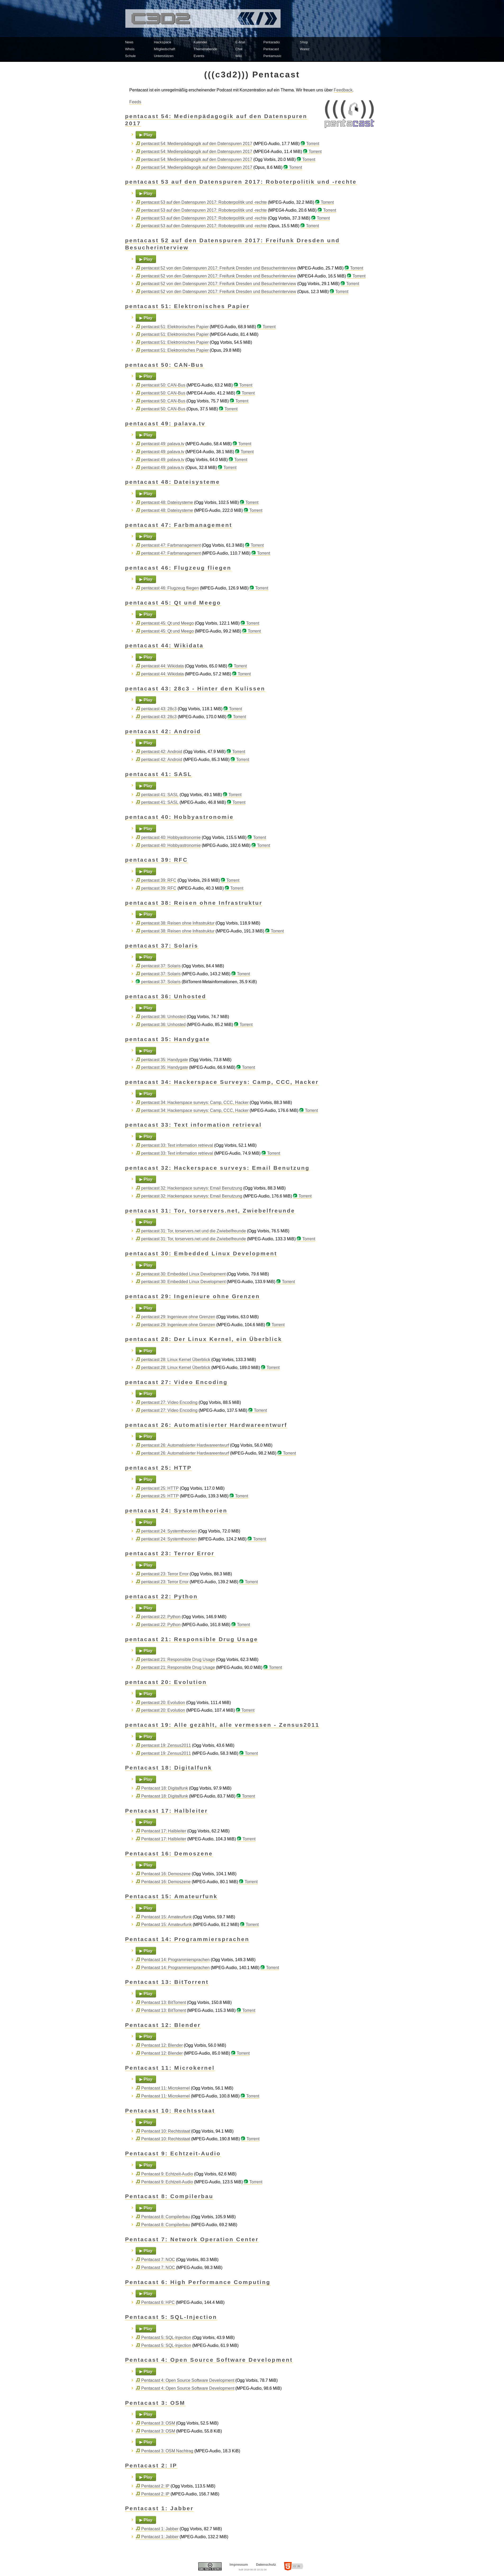
\includegraphics[height=0.2\textheight]{img/pentacast.png}	
		\vspace{0.4cm}

		\underline{c3d2.de/radio.html}
	\end{center}
\end{frame}	

\begin{frame}	
	\frametitle{Chaos Computer Club Dresden}
	\begin{center}
		
\includegraphics[height=0.2\textheight]{img/cms-text.png}
		\vspace{0.4cm}

		c3d2.de/schule.html
	\end{center}
\end{frame}	


\section{CmS}
\subsection{}

\begin{frame}
	\begin{center}
    	
\includegraphics[height=0.5\textheight]{img/cms-text.png}
    \end{center}
\end{frame}
  
\begin{frame}
	\frametitle{Chaos macht Schule}
	\begin{itemize}
		\item<1-> seit ca. 2007
		\item<2-> Ehrenamtlich organisiert
		\item<3-> Bildung und Sensibilisierung
	\end{itemize}
\end{frame}
  
\begin{frame}
	\frametitle{Zielgruppe}
	\begin{itemize}
		\item<1-> Schüler*innen
		\item<2-> Lehrer*innen
		\item<3-> Eltern 
	\end{itemize}
\end{frame}


\begin{frame}
	\frametitle{Inhalte}
	\begin{itemize}
		\item<1-> Datenschutz statt Überwachung
			\only<1>{
				\begin{center}
				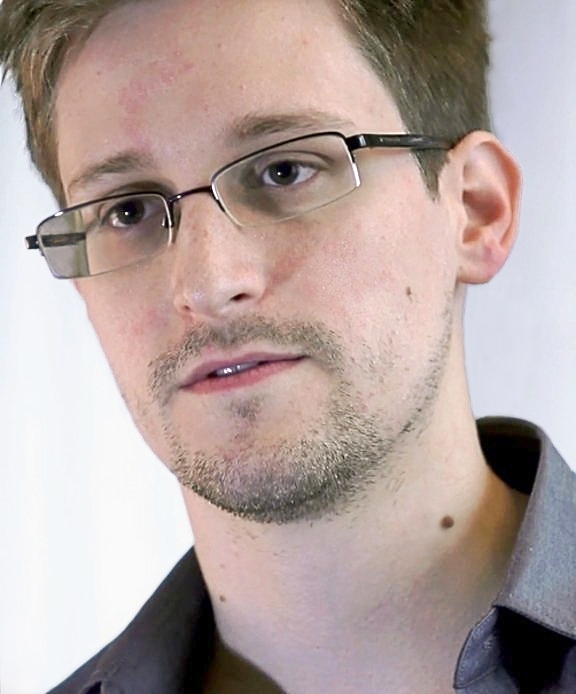
\includegraphics[height=0.7\textheight]{img/snowden.jpg}
				\end{center}
			}
			\only<2>{
				\begin{center}
				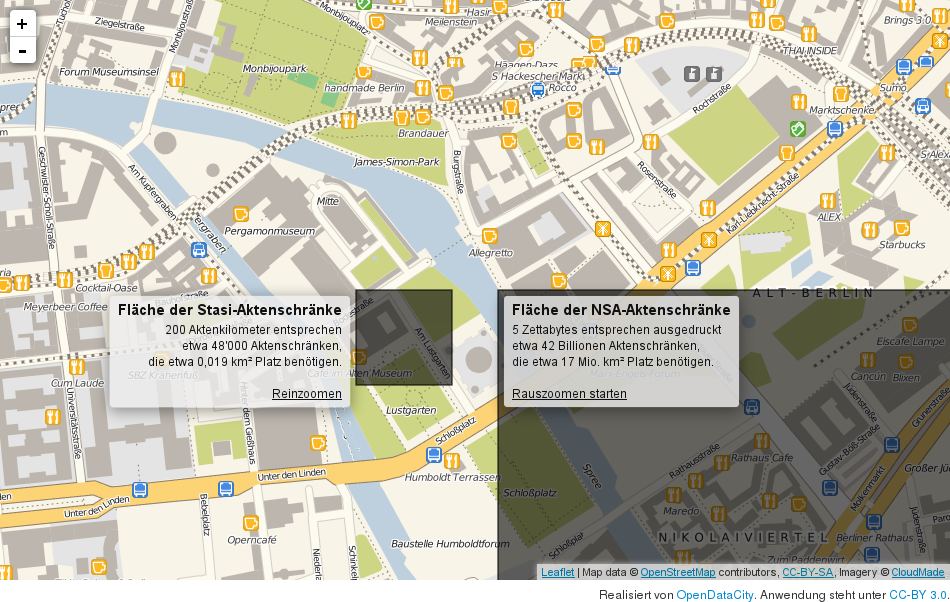
\includegraphics[height=0.7\textheight]{img/akten1.png}
				\end{center}
			}
			\only<3>{
				\begin{center}
				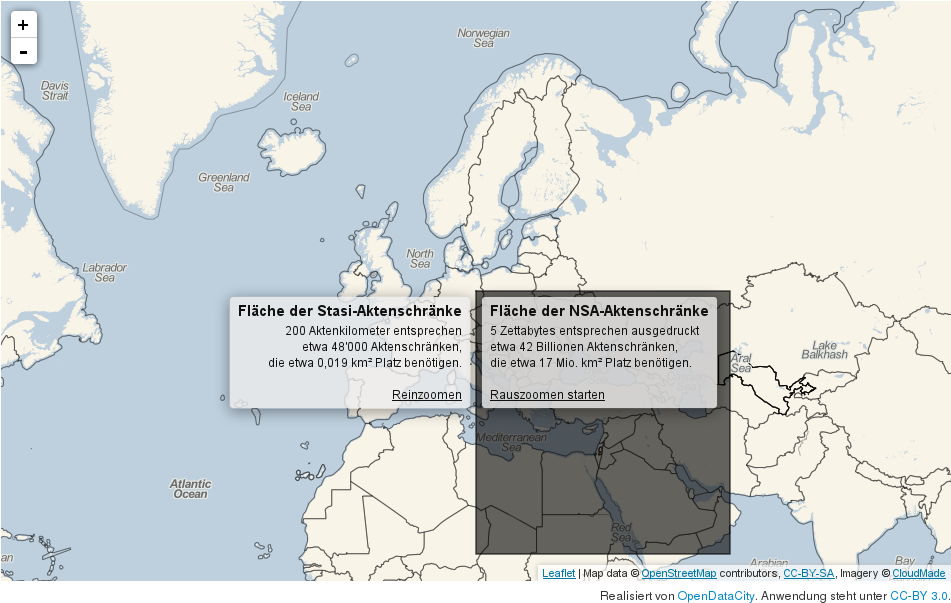
\includegraphics[height=0.7\textheight]{img/akten2.png}
				\end{center}
			}
			\only<4>{
				\begin{center}
				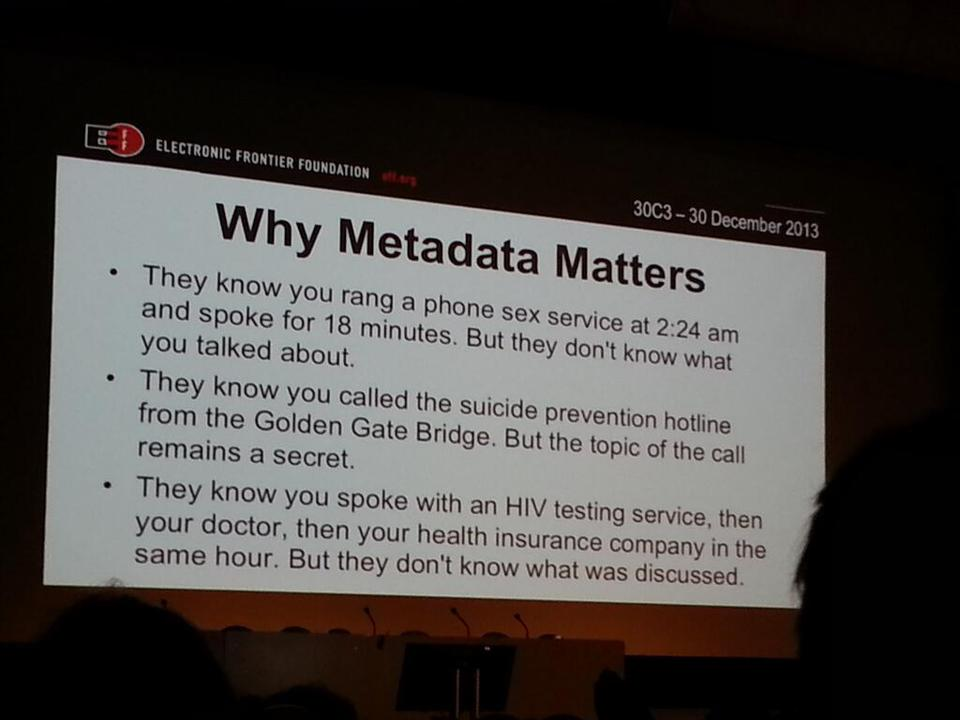
\includegraphics[height=0.7\textheight]{img/metadata-matters.jpg}
				\end{center}
			}
		\item<5-> Sensibilisierung für freie Software \& Dienste
			\only<5>{
				\begin{center}				
				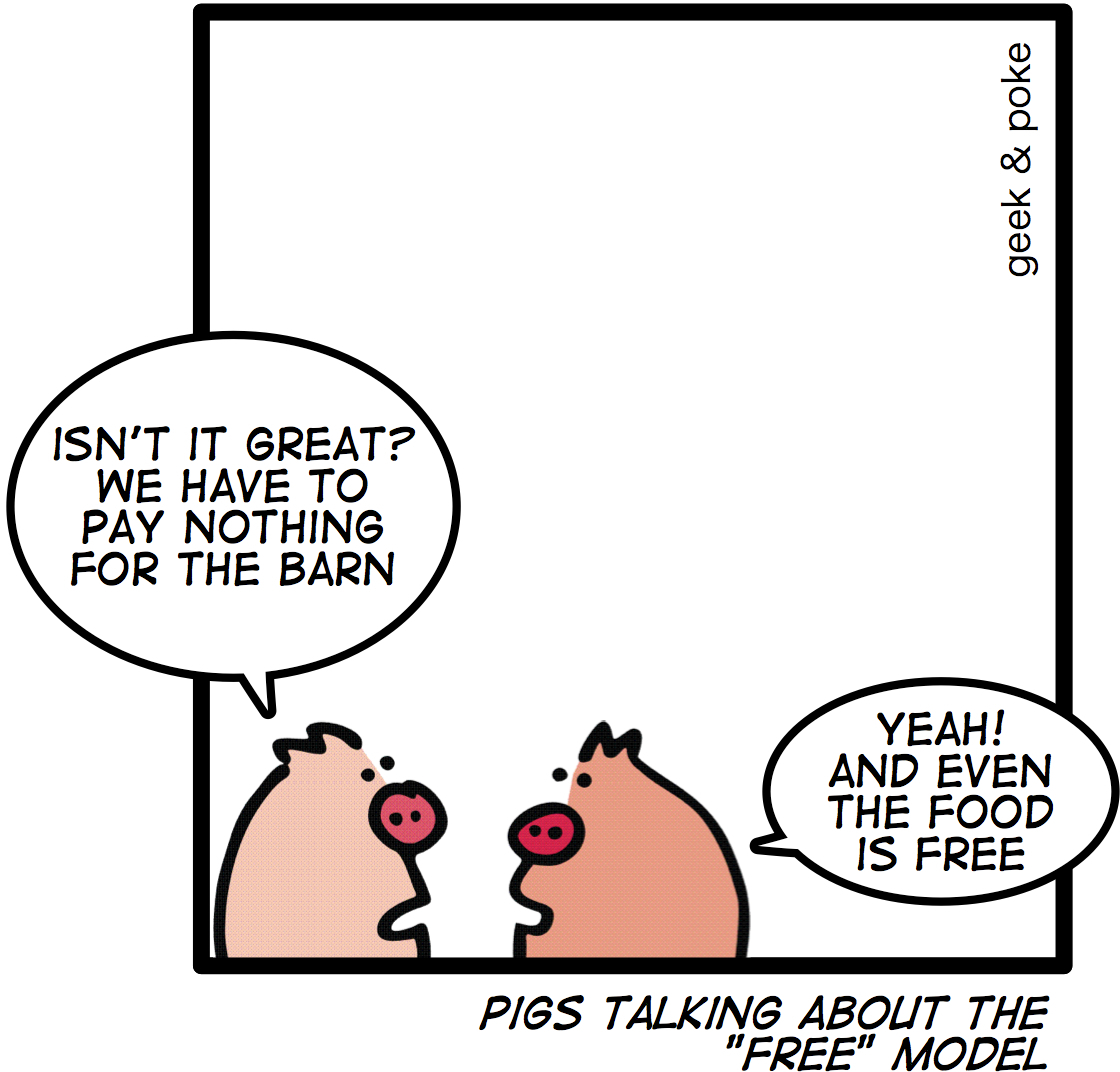
\includegraphics[height=0.7\textheight]{img/business_pigs.jpg}
				\end{center}
			}
		\item<6-> Workshops
			\only<6>{
				\begin{center}
				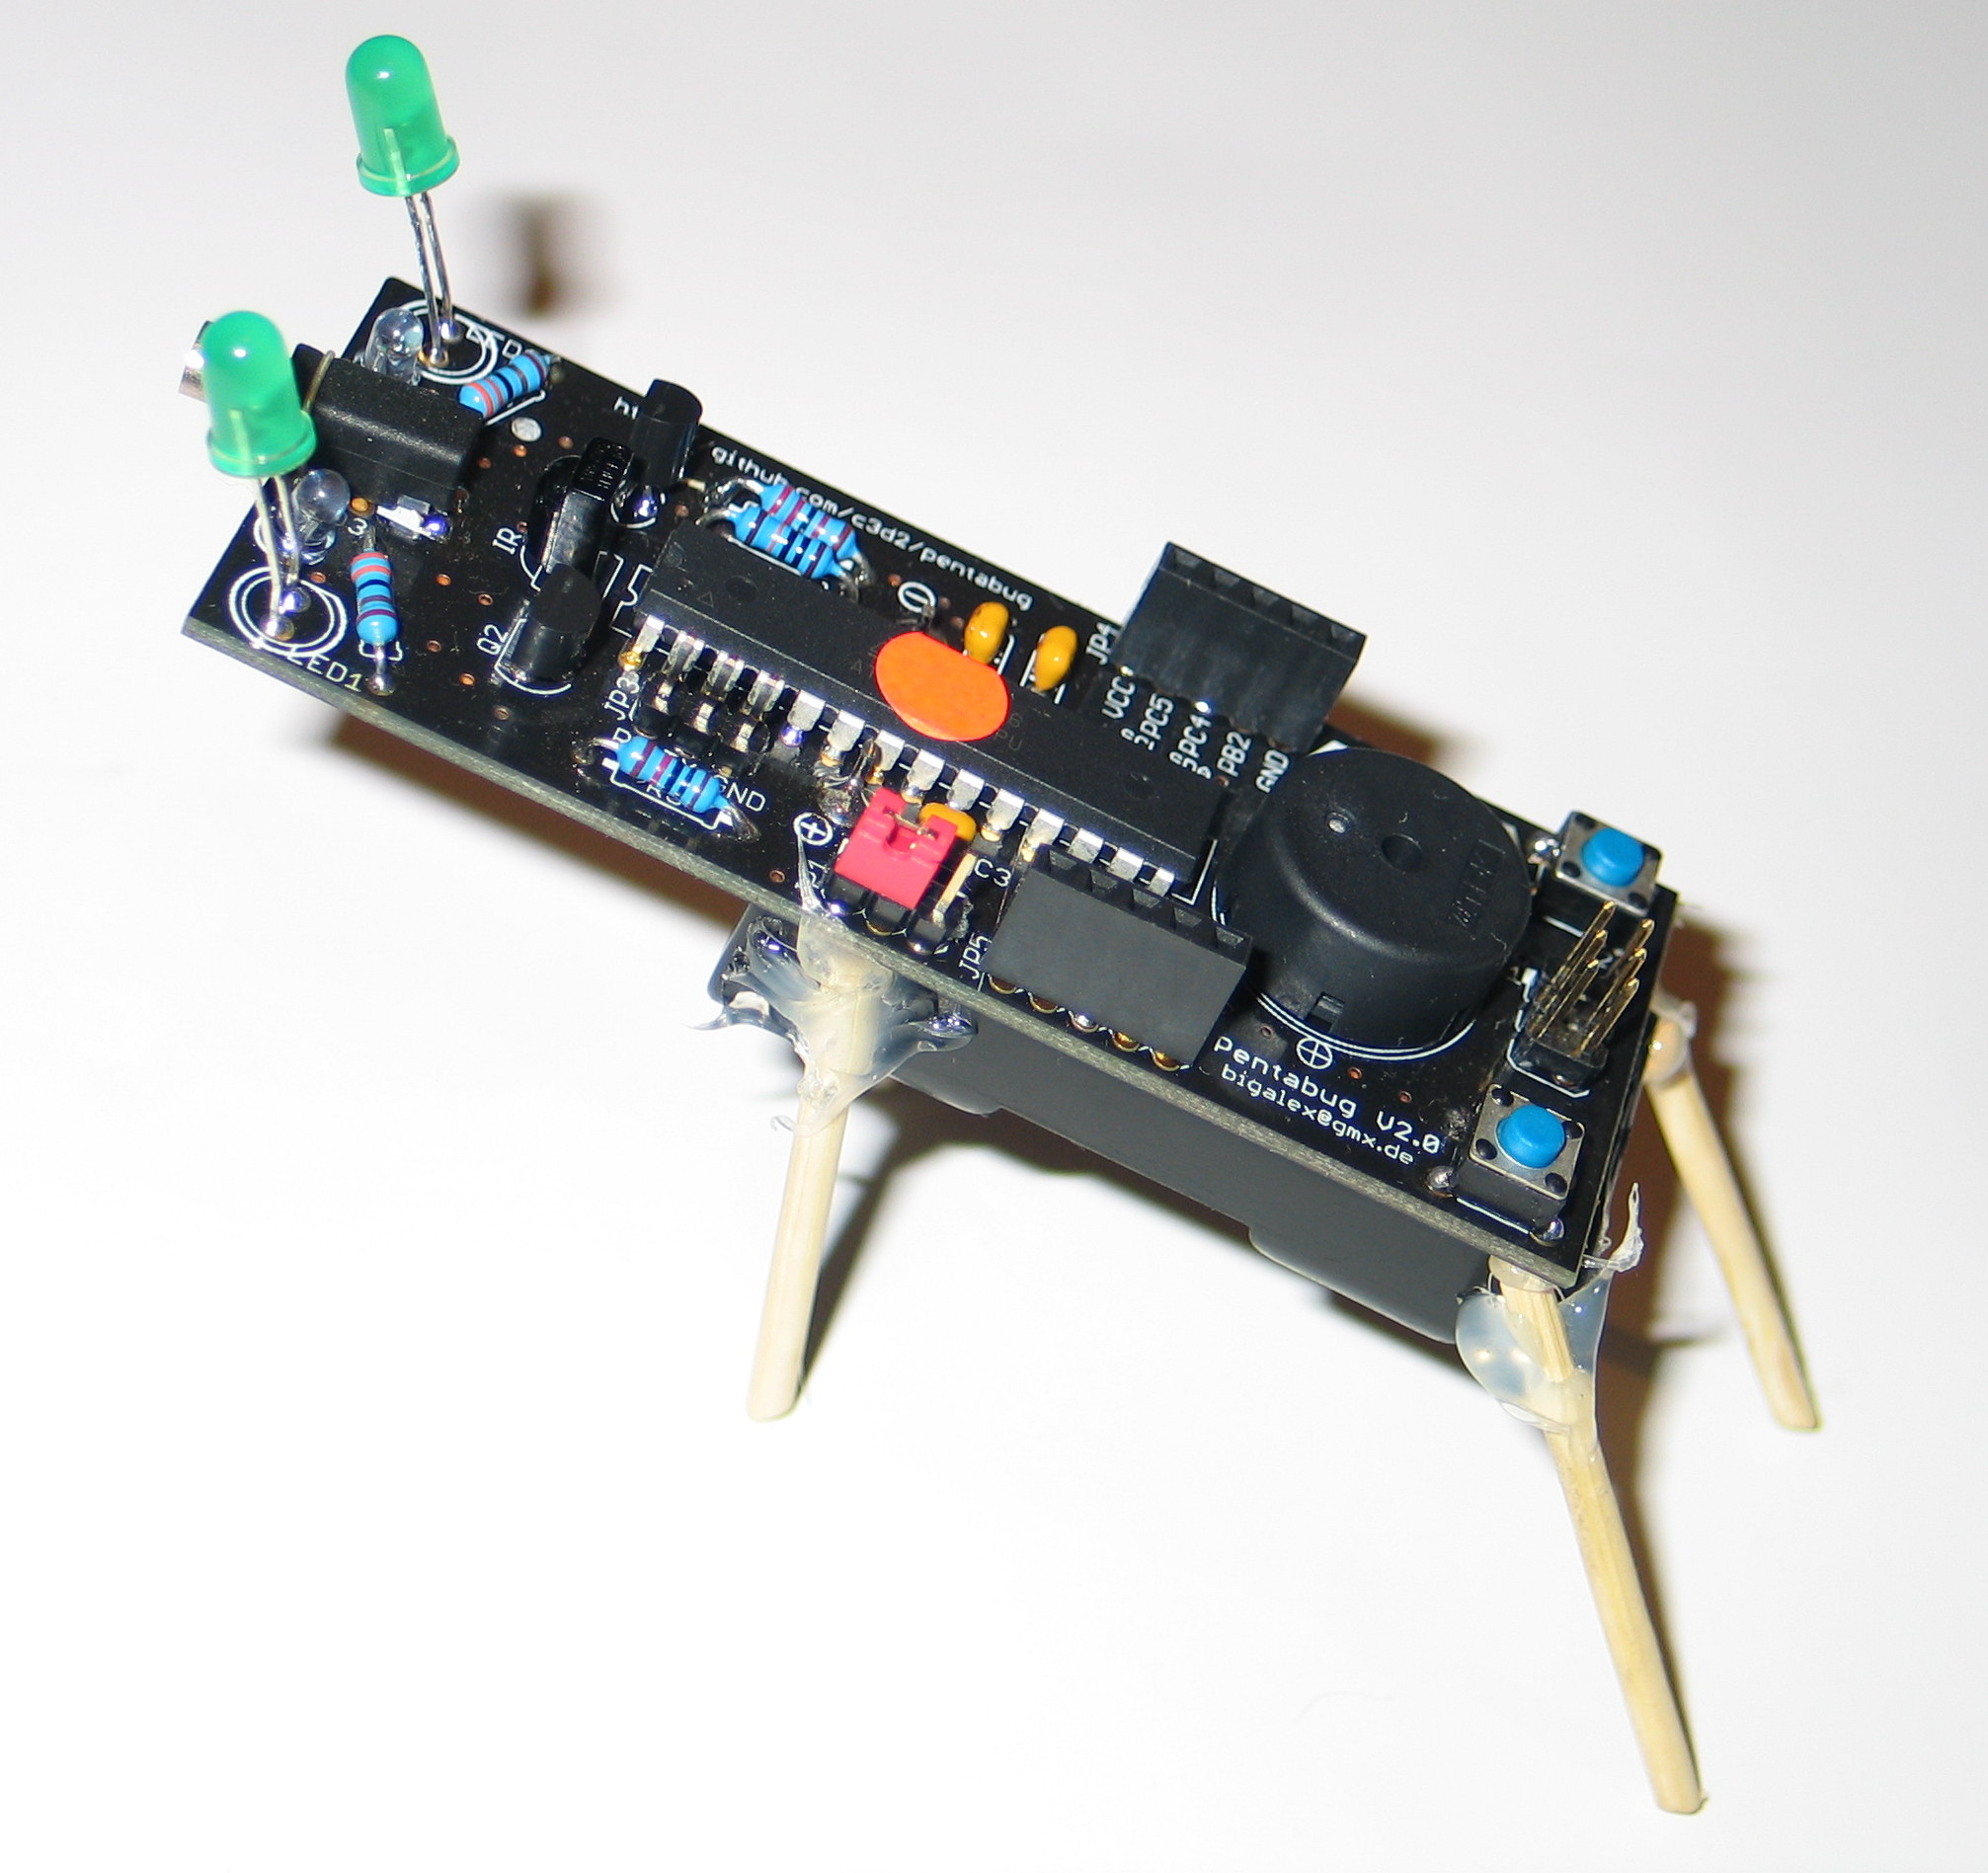
\includegraphics[height=0.5\textheight]{img/pentabug.jpg}
				\end{center}
			}
	\end{itemize}
\end{frame}


\section{Rosenwerk}
	\subsection{}

\begin{frame}
  \frametitle{Rosenwerk}
  \begin{minipage}{\linewidth}
	\centering	
	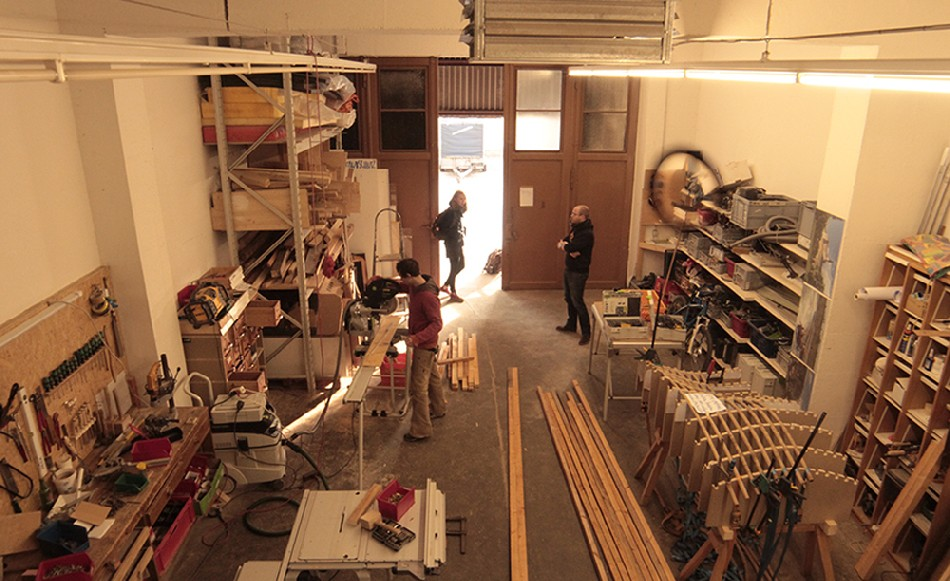
\includegraphics[height=0.6\textheight]{img//rosenwerk-holzwerkstatt-Foto_Carolin_Partsch.jpg}
	\tiny\license{http://www.werkstadtladen.de/rosenwerkoffene-werkstatt/}
	\end{minipage}
  \end{frame}
  \begin{frame}
	\frametitle{Rosenwerk}
	\begin{figure}
	  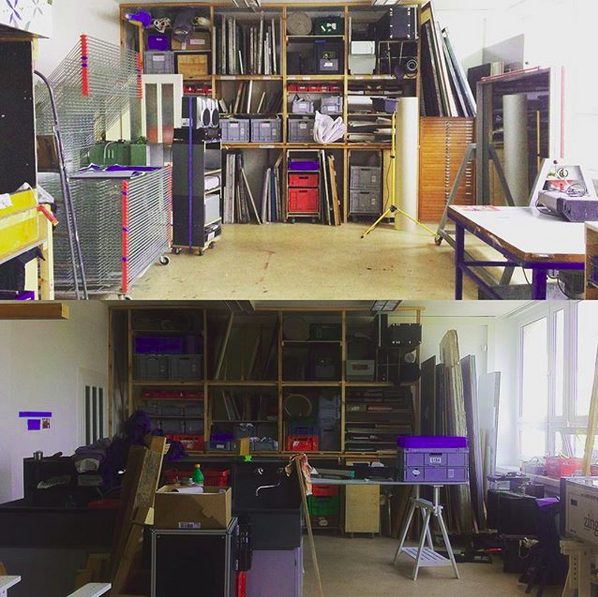
\includegraphics[height=0.7\textheight]{img/rosenwerk-siebdruckwerkstatt.png}
	\end{figure}
  \end{frame}


  \section{SLUB Makerspace}
  \subsection{}
	  
  \begin{frame}
	  \frametitle{SLUB Makerspace}
	  \begin{center}
	  \textbf{S}ächsische 
	  \textbf{L}andesbibliothek – Staats- und 
	  \textbf{U}niversitäts\textbf{b}ibliothek
	  \vspace{20pt}		

	  
\includegraphics[height=0.1\textheight]{img/Logo-SLUB_Farbe.jpg}
	  \end{center}
  \end{frame}
	  
  \begin{frame}
	  \frametitle{SLUB Makerspace}
	  \begin{center}
	  \begin{minipage}{\linewidth}
		  \centering
		  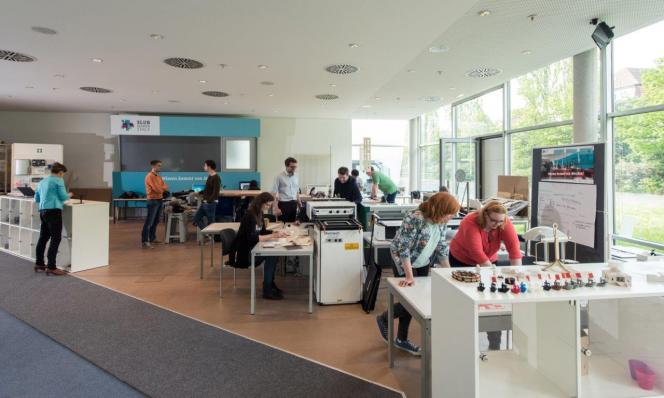
\includegraphics[height=0.7\textheight]{img//slub-makerspace-deutsche-digitale-bibliothek.jpg}
		  \tiny\license{https://www.deutsche-digitale-bibliothek.de/content/saechsische-landesbibliothek-staats-und-universitaetsbibliothek-dresden/}
	  \end{minipage}		
	  \end{center}
  \end{frame}



\section{MKZ}
	\subsection{}

\begin{frame}
  \frametitle{Medienkulturzentrum}
  \begin{minipage}{\linewidth}
	\centering	
	
\includegraphics[height=0.6\textheight]{img//logo_medienkulturzentrum.png}
	
	www.medienkulturzentrum.de
	\end{minipage}
  \end{frame}
  \begin{frame}
	\frametitle{Medienkulturzentrum}
	\begin{minipage}{\linewidth}
		\centering
		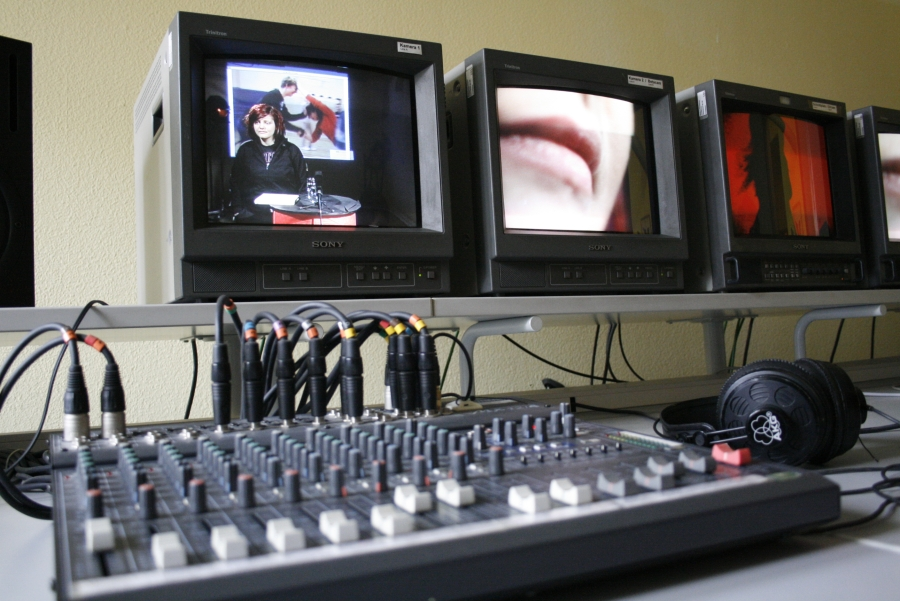
\includegraphics[height=0.7\textheight]{img//mkz-film.jpg}
		\tiny\license{www.medienkulturzentrum.de}
	\end{minipage}
  \end{frame}
  \begin{frame}
	\frametitle{Medienkulturzentrum}
	\begin{minipage}{\linewidth}
		\centering
		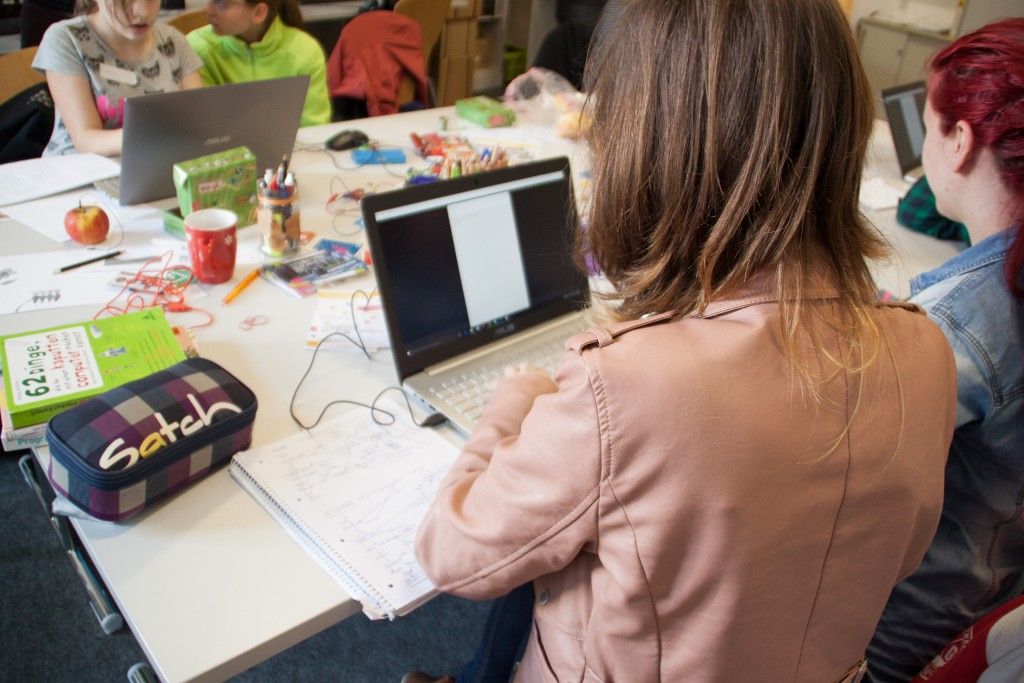
\includegraphics[height=0.7\textheight]{img//medienkulturzentrum-apps-games-coding.jpg}
		\tiny\license{www.medienkulturzentrum.de}
	\end{minipage}
  \end{frame}


  \section{SRZ}
  \subsection{}
	  
	\begin{frame}
		\frametitle{Schülerrechenzentrum}
		\begin{center}
			
\includegraphics[height=0.2\textheight]{img//schuelerrechenzentrum.jpeg}
			\vspace{20pt}		
			
			www.srz.tu-dresden.de
		\end{center}
  	\end{frame}
	  
	\begin{frame}
		\frametitle{Schülerrechenzentrum}
		\begin{center}
		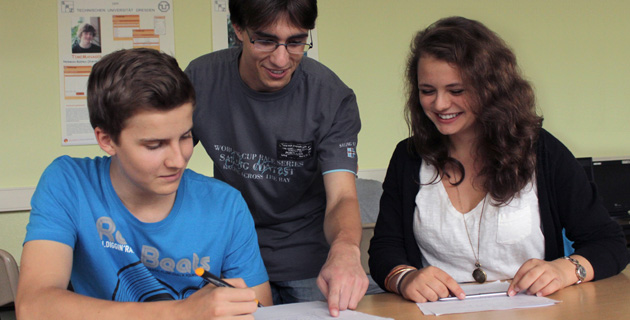
\includegraphics[height=0.6\textheight]{img//schuelerrechenzentrum2.jpg}
		\end{center}
  	\end{frame}


  \section{Events}
  \subsection{}
  \begin{frame}
	\frametitle{Chaos Communication Camp}
	\begin{center}

		
\includegraphics[height=0.2\textheight]{img//camp15-logo.png}
		\vspace{20pt}		
		
		events.ccc.de/camp
	\end{center}
	\end{frame}
	\begin{frame}
		\frametitle{Chaos Communication Camp}
		\begin{minipage}{\linewidth}
			\centering
			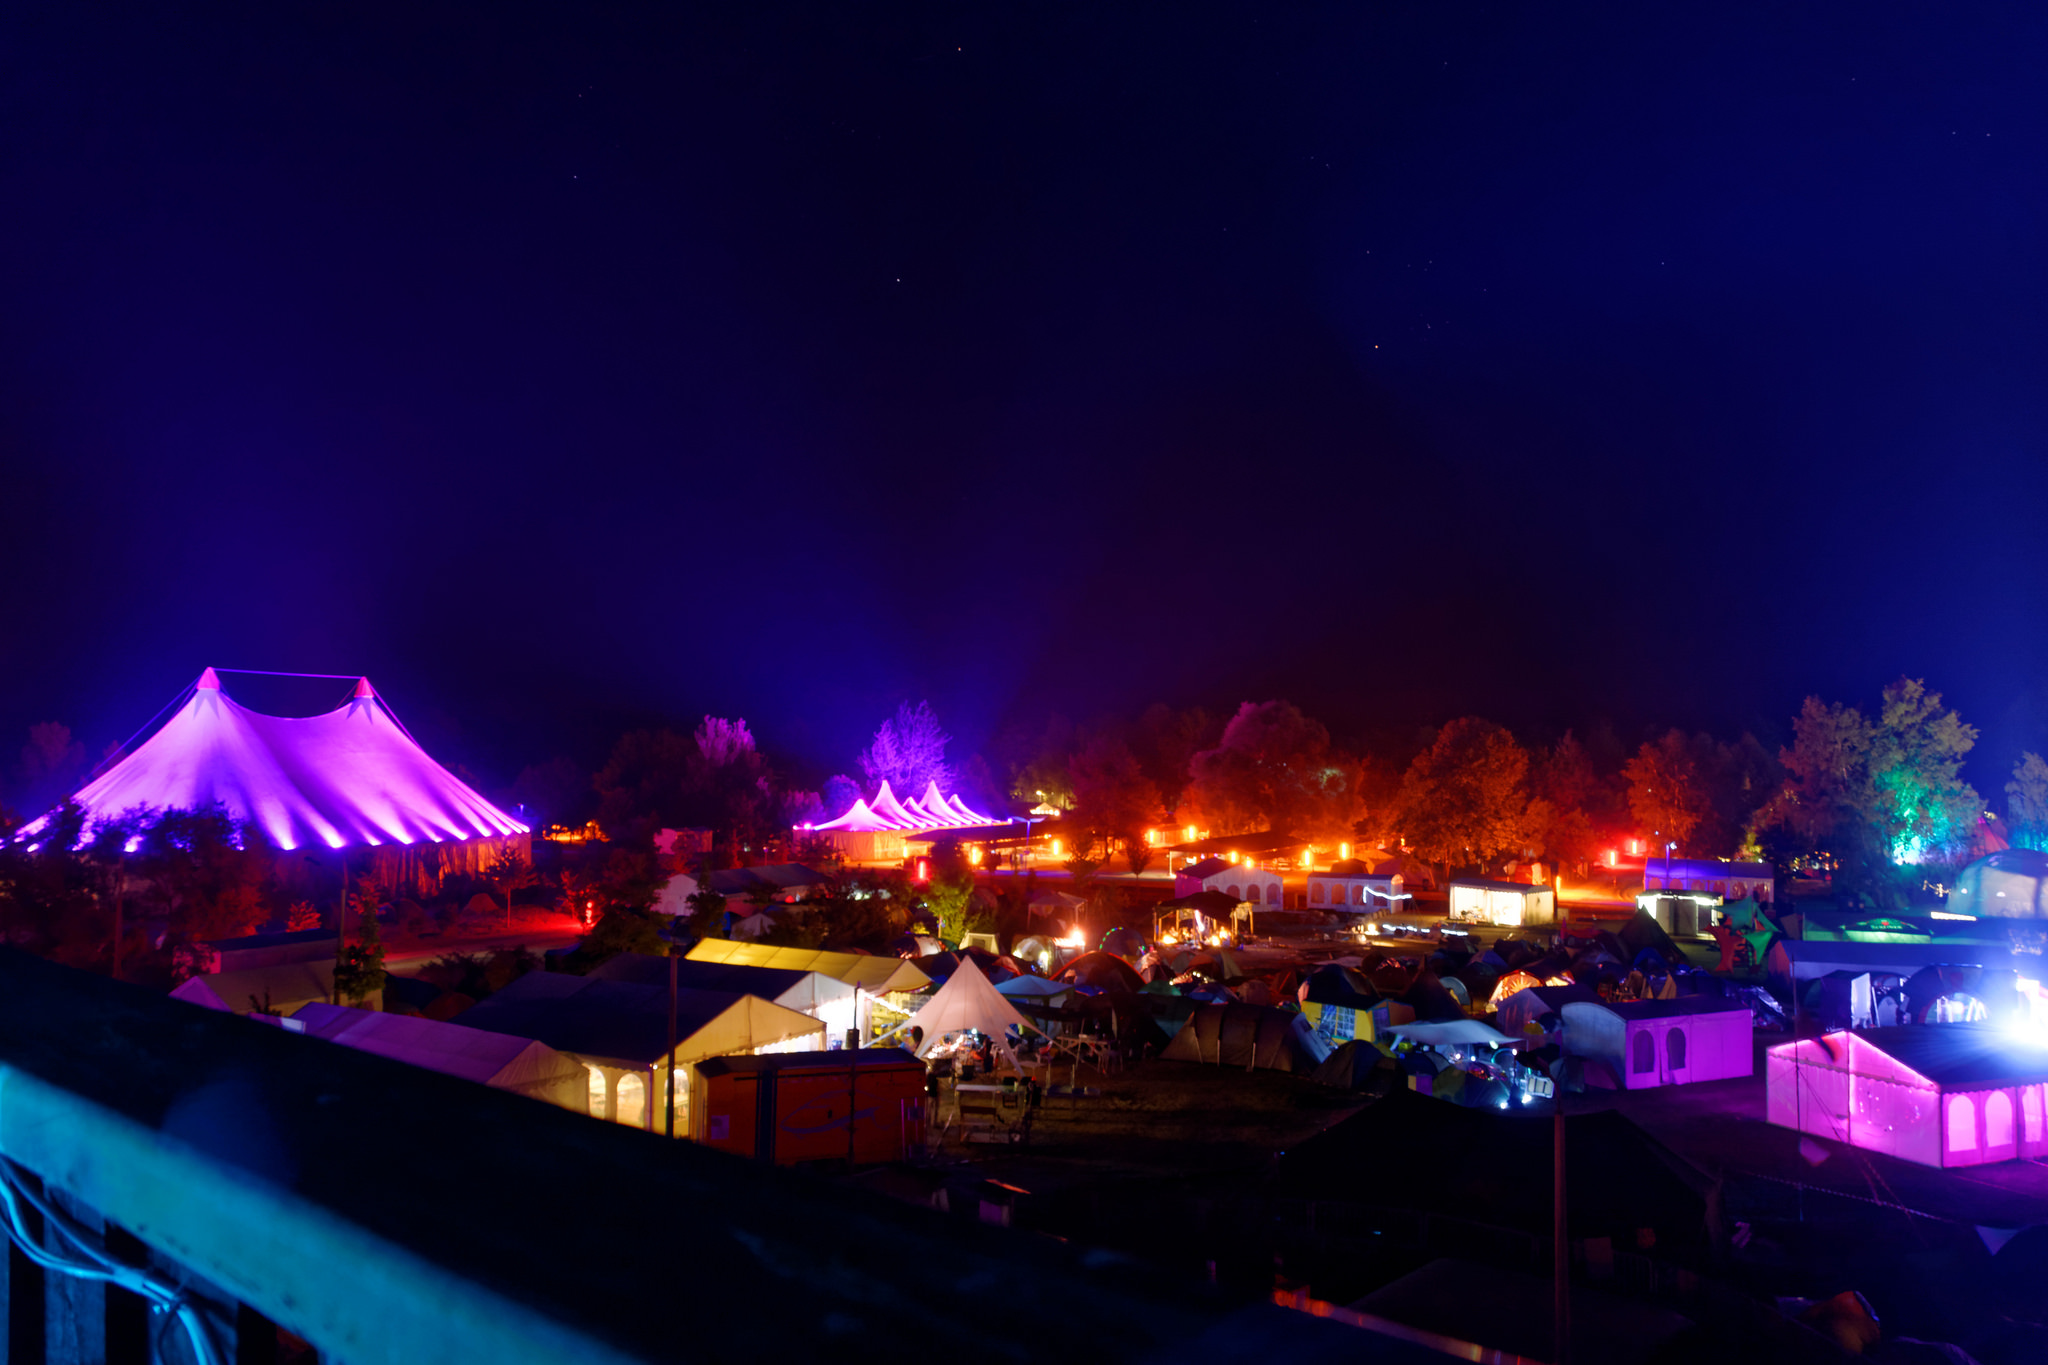
\includegraphics[height=0.7\textheight]{img//camp_flickr_BlinkenArea_org_cc_by_20.jpg}
			\tiny\license{https://www.flickr.com/photos/blinkenarea/20547178111/in/album-72157656744791999/}
		\end{minipage}
	\end{frame}
	\begin{frame}
		\frametitle{Chaos Communication Camp}
		\begin{minipage}{\linewidth}
			\centering
			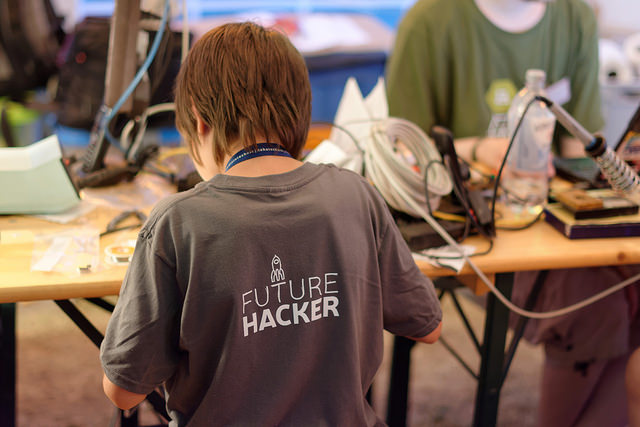
\includegraphics[height=0.7\textheight]{img//camp2015-future-hacker.jpg}
			\tiny\license{https://secure.flickr.com/photos/blinkenarea/20632120901/}
		\end{minipage}
	\end{frame}
	\begin{frame}
		\frametitle{Chaos Communication Camp}
		\begin{minipage}{\linewidth}
			\centering
			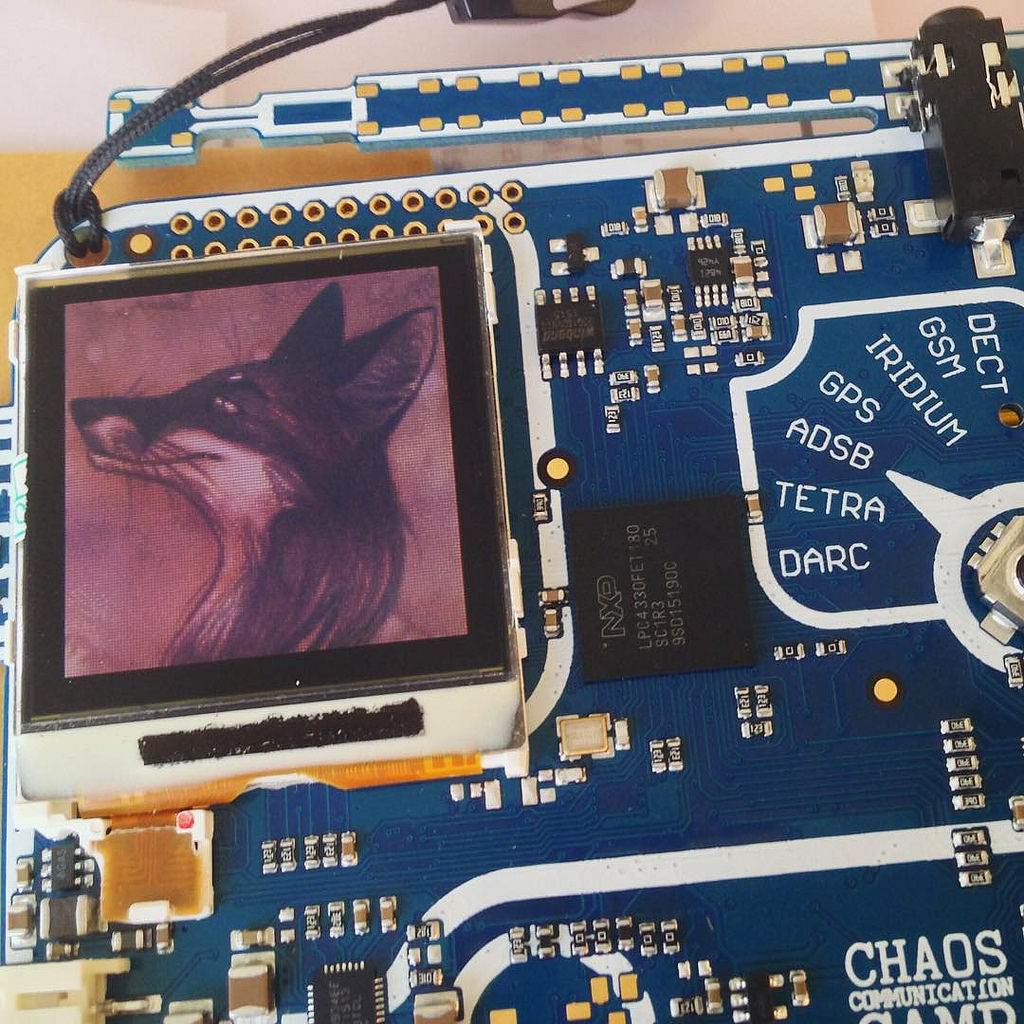
\includegraphics[height=0.7\textheight]{img//camp2015-badge.jpg}
			\tiny\license{https://secure.flickr.com/photos/optikfluffel/19952406623/}
		\end{minipage}
	\end{frame}

	\begin{frame}
		\frametitle{Chaos Communication Congress}
		\begin{center}
			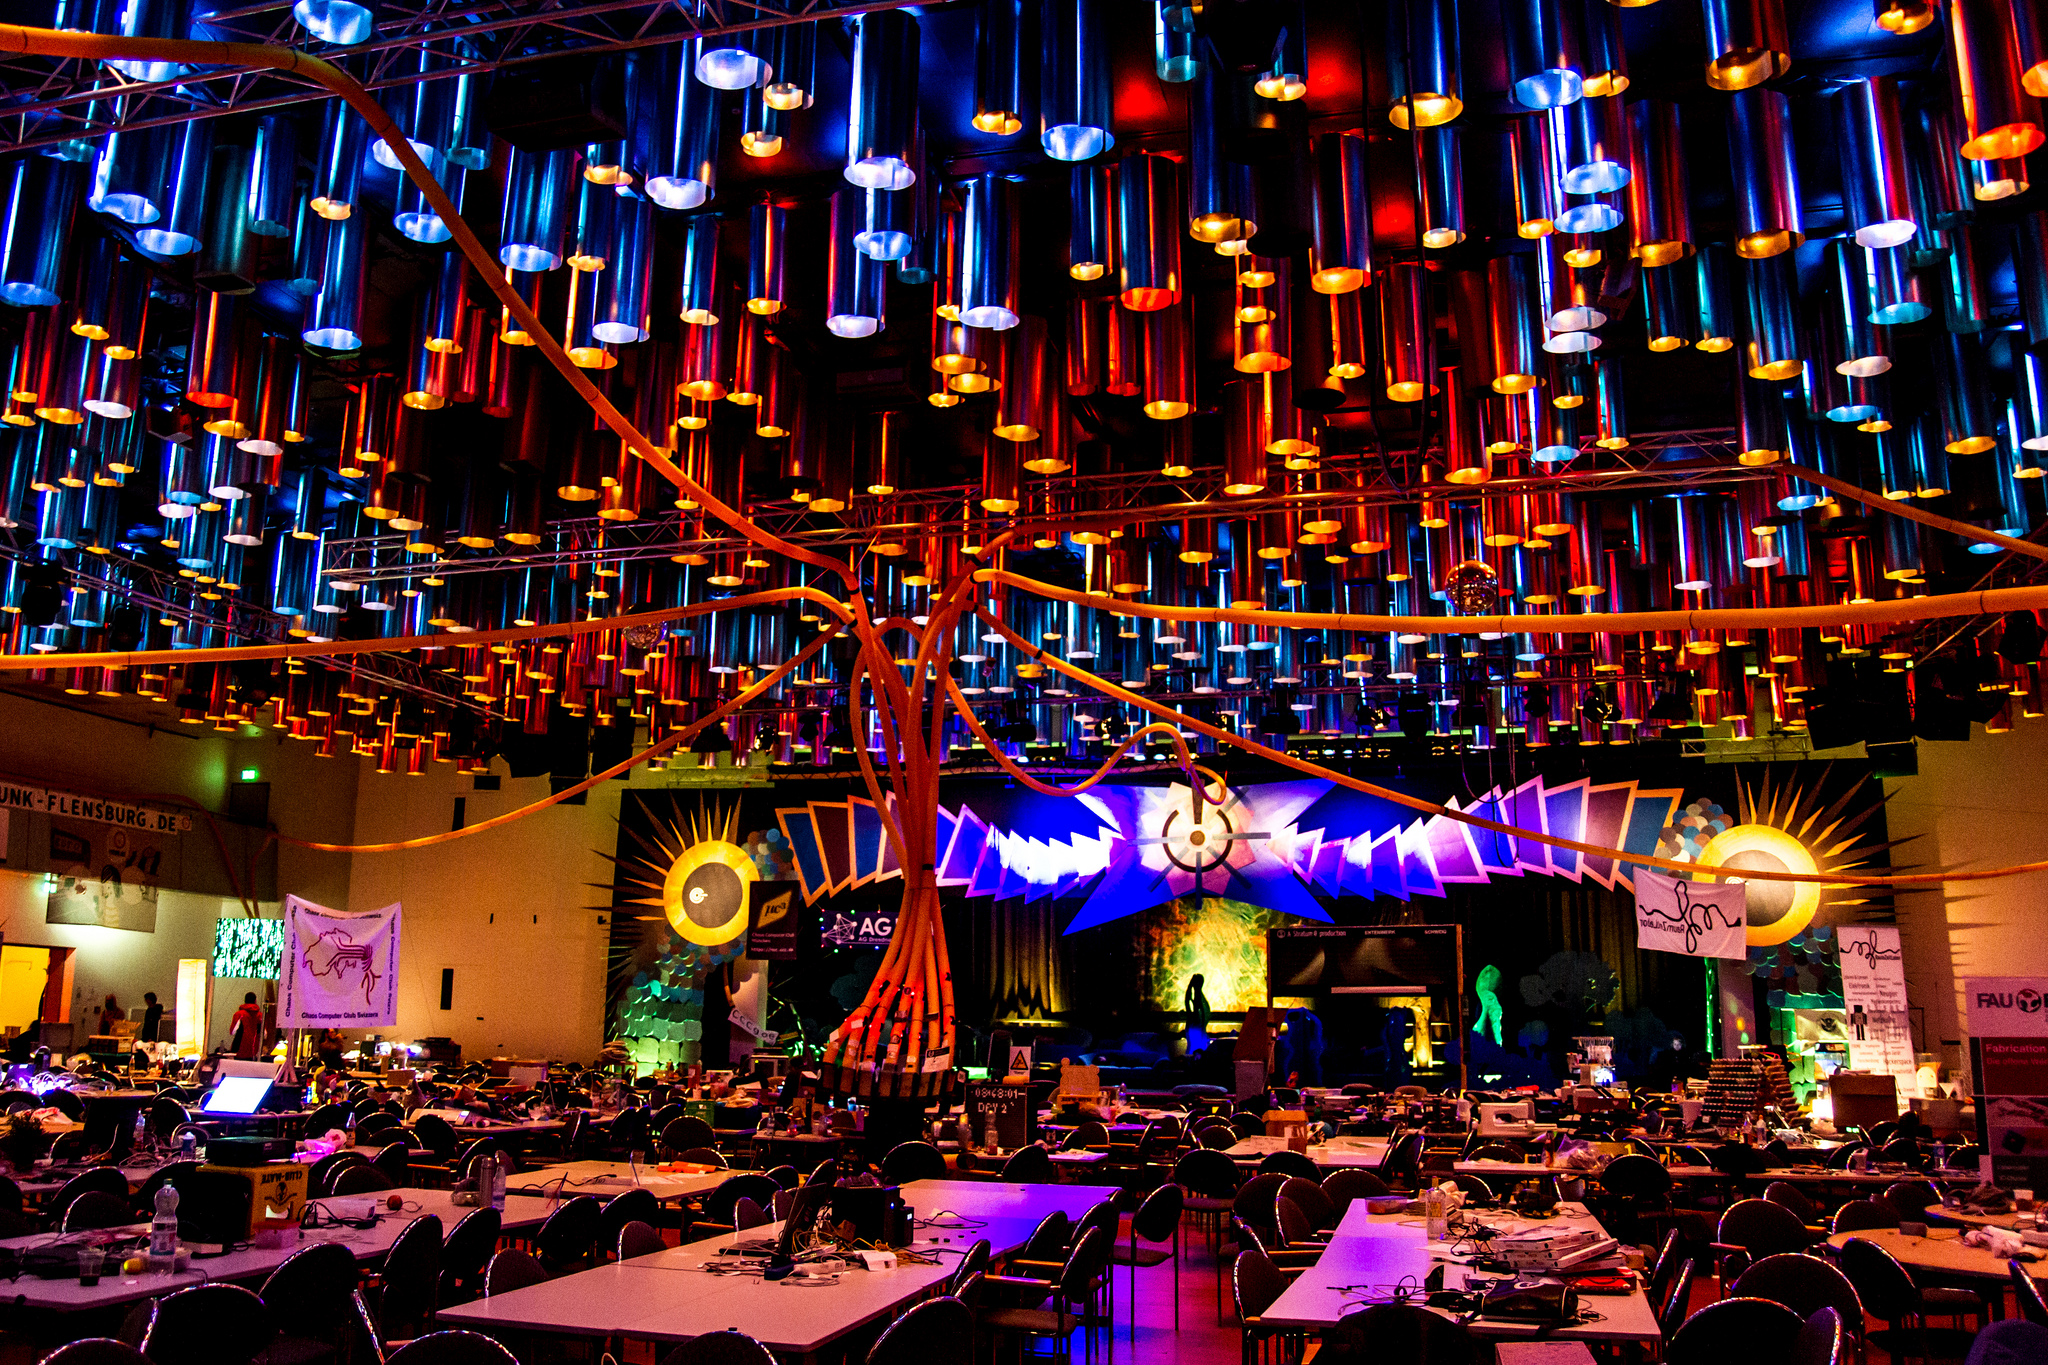
\includegraphics[height=0.2\textheight]{img//congress_flickr_Willi_Thiel_cc_by-nc-sa_2.0.jpg}
			\vspace{20pt}		
			
			events.ccc.de
		\end{center}
		\end{frame}
		\begin{frame}
			\frametitle{Chaos Communication Congress}
			\begin{center}
				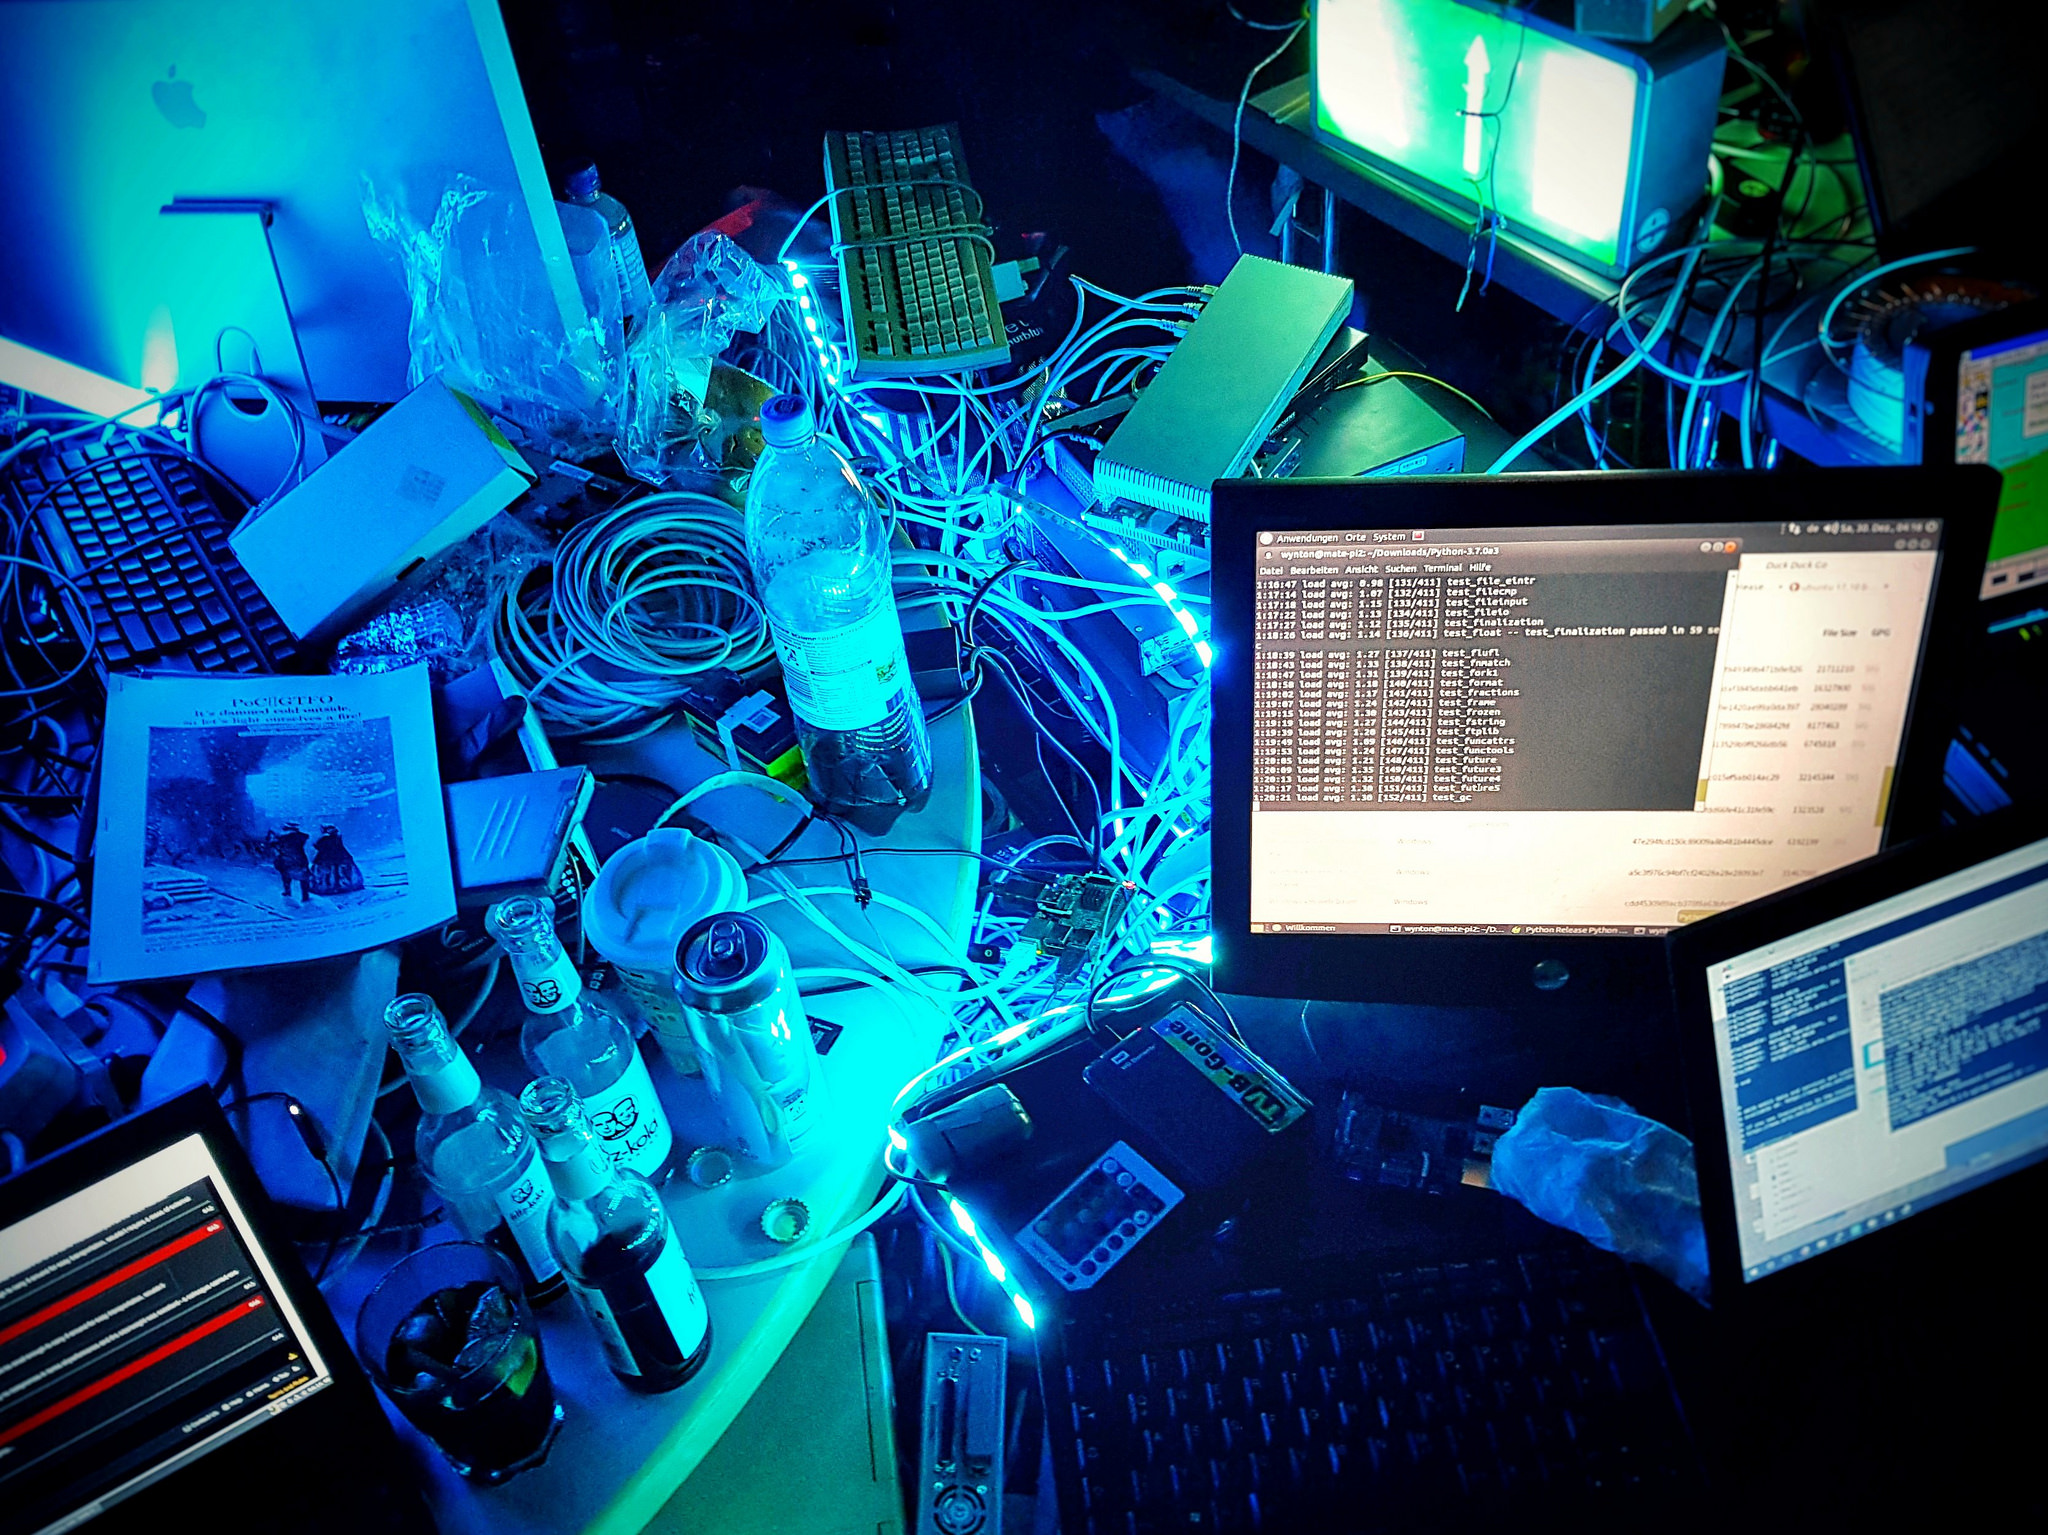
\includegraphics[height=0.7\textheight]{congress-chaos.jpg}
			\end{center}
	\end{frame}	
		
	\begin{frame}
		\frametitle{Deutscher Multimediapreis mb21}
		\begin{center}
			
\includegraphics[height=0.6\textheight]{img//Logo_mb21_weltkugel.jpg}
			\vspace{20pt}		
			
			http://www.mb21.de
		\end{center}
	\end{frame}
	\begin{frame}
		\frametitle{Deutscher Multimediapreis mb21}
		\begin{center}
			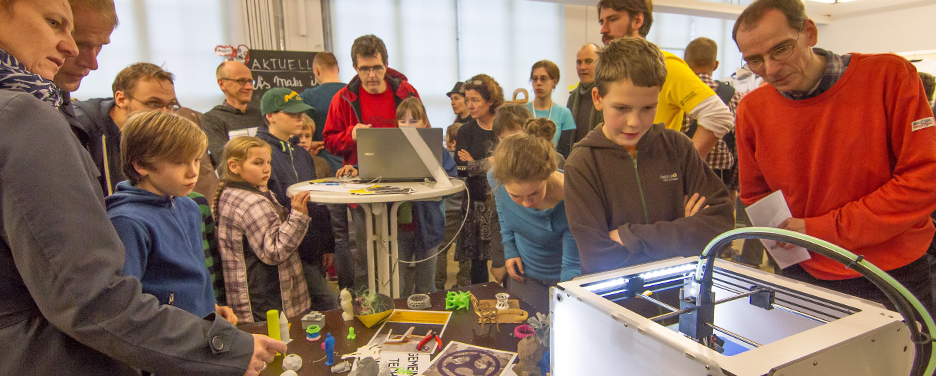
\includegraphics[height=0.6\textheight]{img//mb21_festival.jpg}

			10. und 11. November 

			Technische Sammlungen Dresden
		\end{center}
	\end{frame}

  
	\begin{frame}
		\frametitle{CodeWeek EU}
		\begin{center}
			
\includegraphics[height=0.2\textheight]{img//codeweekeu.png}
			\vspace{20pt}		
			
			https://codeweek.eu
		\end{center}
	\end{frame}
	\begin{frame}
		\begin{center}
			
\includegraphics[height=0.7\textheight]{img//codeweek.png}
		\end{center}
	\end{frame}		
			


	
	  	  

\end{document}
